%%%%%%%%%%%%%%%%%%%%%%%%%%%%%%%%%%%%%%%%%%%%%%%%%%%%%%%%%%%%%%%%%%%%%%%%%%%%%%%%%%%%%%%%%
% BrainSeg-XAI: Hệ thống Phân đoạn Khối u Não và Trí tuệ Nhân tạo Có thể Giải thích
% Lớp Kỹ thuật Điện tử và Tin học K68 - Khoa Vật lý
% Trường Đại học Khoa học Tự nhiên, ĐHQGHN
%%%%%%%%%%%%%%%%%%%%%%%%%%%%%%%%%%%%%%%%%%%%%%%%%%%%%%%%%%%%%%%%%%%%%%%%%%%%%%%%%%%%%%%%%


%----------------------------------------------------------------------------------------
%	PHẦN 1: CÁC PACKAGE CƠ BẢN VÀ CÁC TÙY CHỈNH VĂN BẢN
%----------------------------------------------------------------------------------------

\documentclass[
12pt,
oneside,
english,
doublespacing,
nolistspacing,
liststotoc,
parskip,
headsepline,
chapterinoneline,
]{HUSdissertation}

\usepackage[utf8]{vietnam}

\usepackage{mathptmx}
\usepackage{amsmath}
\usepackage{amssymb}
\allowdisplaybreaks

\usepackage[backend=bibtex,style=numeric,citestyle=ieee,natbib=true]{biblatex}

\addbibresource{main.bib}

\usepackage[autostyle=true]{csquotes}


%----------------------------------------------------------------------------------------
%	PHẦN 2: CÁC PACKAGE BỔ TRỢ THÊM VÀO TRONG QUÁ TRÌNH BIÊN SOẠN
%----------------------------------------------------------------------------------------

\newcommand\ttb{\bfseries\ttfamily}
\RequirePackage{setlst}

\usepackage{multirow}
\usepackage{subfigure}
\usepackage[fontsize=13pt]{scrextend}

\usepackage{titlesec}

\titleformat{\section}
{\normalfont\fontsize{13}{13}\bfseries}{\thesection}{1em}{}

\titleformat{\subsection}
{\normalfont\fontsize{13}{13}\bfseries\itshape}{\thesubsection}{1em}{}

\usepackage{fancyvrb}
\fvset{tabsize=4,vspace=0pt,fontsize=\footnotesize}

\usepackage{longtable}

\usepackage[figuresright]{rotating}
\usepackage{tabularx}

\usepackage{fontawesome5}

\usepackage{tikz}
\usetikzlibrary{calc}

\usepackage{indentfirst}
\setlength{\parindent}{0.5cm}

\usepackage{dirtree}


%----------------------------------------------------------------------------------------
%	PHẦN 3: THÔNG TIN VỀ TIỂU LUẬN
%----------------------------------------------------------------------------------------

\thesistitle{BrainSeg-XAI: Hệ thống Phân đoạn Khối u Não từ Ảnh MRI sử dụng Học Sâu và Trí tuệ Nhân tạo Có thể Giải thích}

\supervisor{GS.TS. Nguyễn Thế Toàn}
\supervisorr{CN. Vi Anh Quân}

\field{Ngành Kỹ thuật Điện tử và Tin học}
\program{Chương trình đào tạo chuẩn}
\doctype{Đề tài Nhập môn Trí tuệ nhân tạo}

\university{\href{http://hus.vnu.edu.vn}{Trường Đại học Khoa học Tự nhiên}}
\department{\href{http://hus.vnu.edu.vn/gioi-thieu/co-cau-to-chuc/khoa-truc-thuoc/khoa-vat-ly.html}{Khoa Vật lý}}

\AtBeginDocument{
	\hypersetup{pdftitle=\ttitle}
	% \hypersetup{pdfauthor=\authorname}
}


\begin{document}

\lstset{style=codePython}

\frontmatter

\pagestyle{plain}


%----------------------------------------------------------------------------------------
%	PHẦN 4: TRANG TIÊU ĐỀ/TRANG BÌA
%----------------------------------------------------------------------------------------

\include{main-cover}
\include{sub-cover}


%----------------------------------------------------------------------------------------
%	PHẦN 5: DANH NGÔN
%----------------------------------------------------------------------------------------

\vspace*{0.2\textheight}

\noindent\enquote{\itshape
	The goal is to turn data into information, and information into insight.
}\bigbreak

\hfill Carly Fiorina


%----------------------------------------------------------------------------------------
%	PHẦN 6: LỜI CẢM ƠN
%----------------------------------------------------------------------------------------

\begin{acknowledgements}
	\addchaptertocentry{\acknowledgementname}
	\thispagestyle{empty}

	Em xin bày tỏ lòng biết ơn chân thành đến giảng viên hướng dẫn, người đã tận tình định hướng và hỗ trợ em trong suốt quá trình thực hiện tiểu luận này.

	Đề tài \textit{BrainSeg-XAI} là cơ hội để em ứng dụng kiến thức học sâu và trí tuệ nhân tạo vào bài toán y tế có giá trị thực tiễn cao: phân đoạn khối u não từ ảnh MRI. Trong quá trình xây dựng hệ thống, em đã học hỏi được nhiều kinh nghiệm quý báu về thiết kế mô hình học sâu, triển khai dịch vụ web, và xây dựng hệ thống AI có khả năng giải thích được kết quả dự đoán.

	Em cũng xin gửi lời cảm ơn đến cộng đồng mã nguồn mở đã cung cấp các thư viện PyTorch, segmentation-models-pytorch, FastAPI và React -- những nền tảng kỹ thuật quan trọng giúp hiện thực hóa ý tưởng của đề tài.

	Em nhận thức rõ những hạn chế còn tồn tại trong bài làm và rất mong nhận được ý kiến đóng góp từ thầy/cô để tiếp tục cải thiện chất lượng nghiên cứu trong tương lai.
\end{acknowledgements}


%----------------------------------------------------------------------------------------
%	PHẦN 7: MỤC LỤC
%----------------------------------------------------------------------------------------

\begin{spacing}{1.15}
	\tableofcontents
\end{spacing}

\begin{spacing}{1.15}
	\listoffigures
\end{spacing}

\begin{spacing}{1.15}
	\listoftables
\end{spacing}


%----------------------------------------------------------------------------------------
%	PHẦN 8: DANH SÁCH TÊN VIẾT TẮT
%----------------------------------------------------------------------------------------

\begin{abbreviations}{ll}

\textbf{AI}    & \textbf{A}rtificial \textbf{I}ntelligence (Trí tuệ nhân tạo)\\
\textbf{XAI}   & e\textbf{X}plainable \textbf{A}rtificial \textbf{I}ntelligence (AI có thể giải thích)\\
\textbf{CNN}   & \textbf{C}onvolutional \textbf{N}eural \textbf{N}etwork (Mạng nơ-ron tích chập)\\
\textbf{MRI}   & \textbf{M}agnetic \textbf{R}esonance \textbf{I}maging (Chụp cộng hưởng từ)\\
\textbf{CAD}   & \textbf{C}omputer-\textbf{A}ided \textbf{D}iagnosis (Chẩn đoán hỗ trợ máy tính)\\
\textbf{Grad-CAM} & \textbf{G}radient-weighted \textbf{C}lass \textbf{A}ctivation \textbf{M}apping\\
\textbf{SMP}   & \textbf{S}egmentation \textbf{M}odels \textbf{P}yTorch\\
\textbf{API}   & \textbf{A}pplication \textbf{P}rogramming \textbf{I}nterface\\
\textbf{GPU}   & \textbf{G}raphics \textbf{P}rocessing \textbf{U}nit\\
\textbf{CPU}   & \textbf{C}entral \textbf{P}rocessing \textbf{U}nit\\
\textbf{LGG}   & \textbf{L}ow-\textbf{G}rade \textbf{G}lioma (U thần kinh độ thấp)\\
\textbf{ReLU}  & \textbf{R}ectified \textbf{L}inear \textbf{U}nit\\
\textbf{BN}    & \textbf{B}atch \textbf{N}ormalization (Chuẩn hóa theo lô)\\
\textbf{CT}    & \textbf{C}omputed \textbf{T}omography (Chụp cắt lớp vi tính)\\
\textbf{PET}   & \textbf{P}ositron \textbf{E}mission \textbf{T}omography\\
\textbf{RGB}   & \textbf{R}ed-\textbf{G}reen-\textbf{B}lue (Không gian màu)\\
\textbf{REST}  & \textbf{RE}presentational \textbf{S}tate \textbf{T}ransfer\\
\textbf{JSON}  & \textbf{J}ava\textbf{S}cript \textbf{O}bject \textbf{N}otation\\

\end{abbreviations}


%----------------------------------------------------------------------------------------
%	PHẦN 9: DANH SÁCH KÝ HIỆU
%----------------------------------------------------------------------------------------

\begin{symbols}{lll}

$x$             & Vector đầu vào của mạng nơ-ron                  & --\\
$\hat{y}$       & Đầu ra dự đoán (logit hoặc xác suất)            & --\\
$y$             & Nhãn thực tế (ground truth mask)                 & --\\
$\sigma(\cdot)$ & Hàm kích hoạt sigmoid                           & --\\
$\mathcal{L}$   & Hàm mất mát (loss function)                     & --\\
$\alpha_k$      & Trọng số Grad-CAM cho kênh đặc trưng $k$        & --\\
$A^k$           & Bản đồ kích hoạt (feature map) kênh $k$         & --\\
$L^{\text{Grad-CAM}}$ & Bản đồ Grad-CAM                           & --\\

\addlinespace

$\text{Dice}$   & Hệ số Dice                                      & --\\
$\text{IoU}$    & Intersection over Union                         & --\\
$P$             & Precision (Độ chính xác)                        & --\\
$R$             & Recall (Độ phủ)                                 & --\\
$S_{\text{risk}}$ & Điểm rủi ro tổng hợp ($0$--$100$)            & --\\

\end{symbols}


%----------------------------------------------------------------------------------------
%	PHẦN 12: NỘI DUNG CÁC CHƯƠNG
%----------------------------------------------------------------------------------------

\mainmatter

\pagestyle{plain}

% MỞ ĐẦU

\chapter*{MỞ ĐẦU}
\addcontentsline{toc}{chapter}{MỞ ĐẦU}

\label{Chapter0}

%----------------------------------------------------------------------------------------

U não là một trong những loại ung thư nguy hiểm nhất với tỷ lệ sống sót sau năm năm thuộc hàng thấp nhất trong nhóm các bệnh ung thư. Chẩn đoán sớm và chính xác đóng vai trò quyết định trong việc lựa chọn phác đồ điều trị và cải thiện tình trạng cho bệnh nhân. Ảnh cộng hưởng từ (MRI) là phương tiện chẩn đoán hình ảnh chủ đạo cho bệnh lý não bộ, song việc phân tích thủ công các lát cắt MRI đòi hỏi nhiều thời gian và phụ thuộc vào kinh nghiệm của bác sĩ chuyên khoa.

Báo cáo này trình bày thiết kế và triển khai hệ thống BrainSeg-XAI -- một hệ thống trí tuệ nhân tạo hỗ trợ chẩn đoán u não từ ảnh MRI, kết hợp khả năng phân đoạn vùng khối u tự động với cơ chế giải thích kết quả dự đoán có thể hiểu được. Hệ thống được xây dựng dựa trên kiến trúc học sâu U-Net và U-Net++, tích hợp kỹ thuật Gradient-weighted Class Activation Mapping (Grad-CAM) để trực quan hóa lý do mô hình đưa ra quyết định, và một bộ máy luật y khoa để đánh giá mức độ rủi ro lâm sàng.

Đề tài thuộc lĩnh vực giao thoa giữa học máy, thị giác máy tính và tin học y tế -- ba lĩnh vực đang có sự phát triển mạnh mẽ trong bối cảnh ứng dụng trí tuệ nhân tạo vào thực tiễn lâm sàng.

% Chương 1: Tổng quan đề tài

\chapter{Tổng quan đề tài}

\label{Chapter1}

\newcommand{\keyword}[1]{\textbf{#1}}
\newcommand{\tabhead}[1]{\textbf{#1}}
\newcommand{\code}[1]{\texttt{#1}}
\newcommand{\file}[1]{\texttt{\bfseries#1}}
\newcommand{\option}[1]{\texttt{\itshape#1}}

%----------------------------------------------------------------------------------------

\section{Bối cảnh và động lực nghiên cứu}

U não là nhóm bệnh lý ác tính có tỷ lệ tử vong cao và diễn tiến nhanh. U thần kinh đệm độ cao (glioblastoma multiforme, GBM) có trung vị thời gian sống sau chẩn đoán chỉ khoảng 14--16 tháng ngay cả khi được phẫu thuật, xạ trị và hóa trị kết hợp \cite{Menze2015}. Ở nhóm u thần kinh đệm độ thấp (LGG), tiên lượng khả quan hơn song bệnh nhân vẫn đối mặt với nguy cơ tiến triển sang thể ác tính cao. Thời điểm phát hiện bệnh đóng vai trò then chốt: u được chẩn đoán ở giai đoạn sớm, khi kích thước còn nhỏ và chưa xâm lấn các cấu trúc quan trọng, cho phép can thiệp triệt để hơn và cải thiện tiên lượng đáng kể.

Ảnh cộng hưởng từ (MRI) là phương tiện hình ảnh học được lựa chọn hàng đầu để đánh giá bệnh lý não bộ nhờ độ tương phản mô mềm vượt trội so với CT và khả năng hiển thị rõ ranh giới khối u. Một nghiên cứu MRI não điển hình có thể bao gồm hàng chục đến hàng trăm lát cắt với nhiều chuỗi xung khác nhau (T1, T2, FLAIR, T1 tăng cường tương phản), tạo ra khối lượng dữ liệu đáng kể cần được bác sĩ chẩn đoán hình ảnh phân tích thủ công. Với khối lượng công việc thủ công lớn, cùng với sự thiếu hụt nhân lực chuyên khoa tại nhiều cơ sở y tế, đặc biệt ở các nước đang phát triển, tạo ra nhu cầu cấp thiết về công cụ hỗ trợ chẩn đoán tự động.

Các mô hình học sâu và đặc biệt là các mạng nơ-ron tích chập (CNN) đã chứng minh hiệu quả vượt trội trong các bài toán phân tích ảnh y tế \cite{Litjens2017}. Tuy nhiên, một thách thức cơ bản khi triển khai các mô hình học sâu trong lâm sàng là vấn đề ``hộp đen'' (black box): mô hình đưa ra kết quả nhưng không cung cấp giải thích về cơ sở của quyết định. Bác sĩ lâm sàng cần hiểu \textit{tại sao} hệ thống AI đánh dấu một vùng là khối u, chứ không chỉ biết rằng nó là khối u. Đây là điều kiện tiên quyết để AI có thể được chấp nhận và tin tưởng trong thực hành y tế \cite{Doshi2017}.

\begin{figure}[h!]
    \centering
    \subfigure[Ảnh MRI não (T1-Gd, axial)]{
        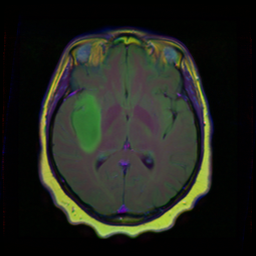
\includegraphics[width=0.30\textwidth]{Figures/Gallery/BrainMRI.png}
    }
    \hspace{4pt}
    \subfigure[Mặt nạ phân đoạn (ground truth)]{
        
\includegraphics[width=0.30\textwidth]{Figures/Gallery/Tumor_Mask.png}
    }
    \hspace{4pt}
    \subfigure[Overlay: vùng khối u (xanh lá)]{
        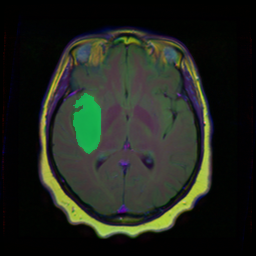
\includegraphics[width=0.30\textwidth]{Figures/Gallery/BrainMRI_overlay.png}
    }
    \caption{Ví dụ một mẫu từ bộ dữ liệu LGG MRI Segmentation \cite{Buda2019}: ảnh MRI gốc (trái), mặt nạ nhị phân do chuyên gia chú thích (giữa) và overlay vùng khối u trên ảnh gốc (phải). Đây là định dạng đầu vào và đầu ra của bài toán phân đoạn tự động.}
    \label{fig:mri_example}
\end{figure}

\section{Tổng quan bài toán}

Bài toán nghiên cứu được xác định như sau:

\textbf{Đầu vào:} Một ảnh MRI não dạng 2D (một lát cắt đơn), định dạng JPEG hoặc PNG, kích thước tùy ý.

\textbf{Yêu cầu xử lý:}
\begin{enumerate}
    \item \textit{Phân đoạn tự động:} Tạo ra mặt nạ nhị phân ($256 \times 256$ pixel) xác định các pixel thuộc vùng khối u.
    \item \textit{Giải thích quyết định:} Tạo ra bản đồ nhiệt Grad-CAM trực quan hóa vùng ảnh ảnh hưởng đến quyết định của mô hình.
    \item \textit{Trích xuất đặc trưng y khoa:} Tính toán các chỉ số hình thái học gồm diện tích, độ bất đối xứng hình dạng, độ phức tạp đường biên, dịch chuyển đường giữa và số vùng khối u.
    \item \textit{Đánh giá rủi ro lâm sàng:} Dựa trên hệ thống phân loại khối cấp độ (grading) của Tổ chức Y tế Thế giới (\textbf{WHO}), phân loại mức độ nguy cơ của khối u phát hiện thành bốn mức: Thấp, Trung bình, Cao, Rất cao.
\end{enumerate}

\textbf{Đầu ra:} Kết quả JSON bao gồm năm ảnh mã hóa base64, vector đặc trưng hình thái và cấu trúc đánh giá rủi ro kèm khuyến nghị lâm sàng.

\section{Các phương pháp hiện nay}

\subsection{Phân đoạn ảnh y tế truyền thống}

Trước khi học sâu trở thành chuẩn mực, phân đoạn ảnh y tế dựa chủ yếu vào các kỹ thuật xử lý ảnh cổ điển: phân ngưỡng Otsu, phân cụm k-means, mô hình đường biên hoạt động (active contour), và phân đoạn dựa trên atlas não bộ. Các phương pháp này đòi hỏi tiền xử lý thủ công đáng kể, nhạy cảm với nhiễu và biến thiên độ tương phản giữa các thiết bị MRI khác nhau.

\subsection{Phương pháp học sâu cho phân đoạn ảnh y tế}

Sự xuất hiện của U-Net \cite{Ronneberger2015} vào năm 2015 tạo ra bước ngoặt trong phân đoạn ảnh y tế. U-Net hoạt động hiệu quả với dữ liệu hạn chế nhờ kiến trúc encoder-decoder đối xứng và skip connections. U-Net++ \cite{Zhou2018} sau đó giới thiệu các skip connections dày đặc lồng nhau (nested), tổng hợp thông tin ở nhiều tỷ lệ không gian. Cuộc thi phân đoạn u não BraTS \cite{Menze2015} đã thúc đẩy sự phát triển mạnh mẽ của các kiến trúc ngày càng sâu hơn, từ nnU-Net cho đến các biến thể dựa trên transformer như SwinUNet.

Thư viện \textit{segmentation-models-pytorch} (SMP) \cite{Yakubovskiy2019} tổng hợp nhiều kiến trúc phân đoạn (U-Net, U-Net++, DeepLabV3+, FPN, MANet) với các encoder pretrained (ResNet, EfficientNet, v.v.) trong một giao diện thống nhất, giảm đáng kể công sức triển khai.

\subsection{Khả năng giải thích trong AI y tế}

Grad-CAM \cite{Selvaraju2017} là kỹ thuật phổ biến nhất để trực quan hóa quyết định của CNN: sử dụng gradient của tín hiệu mục tiêu so với bản đồ đặc trưng (feature map) tại một lớp tích chập nhất định để tạo ra bản đồ nhiệt định vị vùng ảnh quan trọng. Không yêu cầu thay đổi kiến trúc mô hình và áp dụng được cho bất kỳ CNN nào, Grad-CAM trở thành lựa chọn hợp lý cho hệ thống triển khai thực tế.

\section{Mục tiêu và phạm vi nghiên cứu}

\textbf{Mục tiêu chính:}
\begin{itemize}
    \item Xây dựng pipeline end-to-end từ ảnh MRI đầu vào đến kết quả phân đoạn và đánh giá rủi ro.
    \item Tích hợp Grad-CAM để tạo ra giải thích trực quan cho quyết định phân đoạn.
    \item Xây dựng bộ máy luật y khoa chuyển đổi đặc trưng hình thái thành đánh giá rủi ro lâm sàng có cấu trúc.
    \item Triển khai dưới dạng ứng dụng web có thể sử dụng từ trình duyệt.
\end{itemize}

\textbf{Phạm vi nghiên cứu:}
\begin{itemize}
    \item Dữ liệu: bộ dữ liệu LGG MRI Segmentation \cite{Buda2019} gồm 3.929 ảnh MRI não 2D với nhãn phân đoạn.
    \item Mô hình: U-Net thuần và U-Net++ với encoder EfficientNet-B4 pretrained trên ImageNet.
    \item Đầu ra phân đoạn: mặt nạ nhị phân với ngưỡng quyết định 0.5 trên đầu ra sigmoid.
    \item Đánh giá rủi ro mang tính tham khảo lâm sàng, không thay thế chẩn đoán của bác sĩ.
\end{itemize}


% Chương 2: Cơ sở lý thuyết

\chapter{Cơ sở lý thuyết}

\label{Chapter2}

%----------------------------------------------------------------------------------------

\section{Mạng nơ-ron tích chập và học sâu}

\subsection{Tích chập hai chiều}

Phép tích chập là phép toán nền tảng trong CNN. Cho ảnh đầu vào $\mathbf{X} \in \mathbb{R}^{H \times W \times C}$ và bộ lọc (kernel) $\mathbf{K} \in \mathbb{R}^{k \times k \times C \times F}$, đầu ra của một lớp tích chập tại vị trí $(i, j)$ cho kênh đầu ra $f$ là:

\begin{equation}
    Y_{i,j,f} = \sum_{m=0}^{k-1} \sum_{n=0}^{k-1} \sum_{c=0}^{C-1} X_{i+m,\, j+n,\, c} \cdot K_{m,n,c,f} + b_f
    \label{eq:conv2d}
\end{equation}

trong đó $b_f$ là bias và $k$ là kích thước kernel. Sau tích chập, hàm kích hoạt ReLU thường được áp dụng: $\text{ReLU}(x) = \max(0, x)$.

\subsection{Batch Normalization}

Batch Normalization (BN) \cite{Goodfellow2016} chuẩn hóa đầu ra của lớp trước khi áp dụng hàm kích hoạt, giúp ổn định quá trình huấn luyện và cho phép sử dụng learning rate lớn hơn. Với mini-batch $\mathcal{B} = \{x_1, \ldots, x_m\}$:

\begin{equation}
    \hat{x}_i = \frac{x_i - \mu_{\mathcal{B}}}{\sqrt{\sigma_{\mathcal{B}}^2 + \epsilon}}, \qquad
    y_i = \gamma \hat{x}_i + \beta
    \label{eq:batchnorm}
\end{equation}

trong đó $\mu_{\mathcal{B}}$, $\sigma_{\mathcal{B}}^2$ là trung bình và phương sai của batch; $\gamma$, $\beta$ là tham số học được.

\section{Kiến trúc U-Net}

\subsection{Kiến trúc encoder-decoder}

U-Net \cite{Ronneberger2015} được Ronneberger và cộng sự đề xuất năm 2015, ban đầu cho bài toán phân đoạn tế bào kính hiển vi y tế. Kiến trúc bao gồm hai nhánh đối xứng:

\textbf{Encoder (đường giảm mẫu):} Gồm các khối DoubleConv lặp lại, mỗi khối gồm hai lớp tích chập $3 \times 3$ -- BatchNorm -- ReLU, theo sau là MaxPooling $2 \times 2$ để giảm không gian đặc trưng đồng thời tăng số kênh. Mạng đặc biệt trong đề tài này có encoder với bốn bước giảm mẫu, tăng số kênh từ 64 lên 128, 256, 512, rồi 1024.

\textbf{Decoder (đường tăng mẫu):} Sử dụng tích chập chuyển vị (transposed convolution) $2 \times 2$ để tăng gấp đôi không gian đặc trưng, sau đó nối (concatenate) với bản đồ đặc trưng tương ứng từ encoder qua skip connection, cuối cùng áp dụng DoubleConv.

\textbf{Skip connections:} Đây là đặc điểm then chốt của U-Net. Việc ghép nối trực tiếp bản đồ đặc trưng từ encoder sang decoder tương ứng giúp khôi phục chi tiết không gian bị mất trong quá trình giảm mẫu -- điều đặc biệt quan trọng với bài toán phân đoạn yêu cầu độ chính xác pixel.

Lớp đầu ra là tích chập $1 \times 1$ ánh xạ về số kênh bằng số lớp cần phân đoạn (ở đây là 1 cho bài toán phân đoạn nhị phân). Ngưỡng sigmoid $\sigma(\cdot) > 0.5$ xác định pixel là khối u.

Kiến trúc vanilla U-Net trong hệ thống BrainSeg-XAI được định nghĩa tại \texttt{models/unet.py} với các lớp: \texttt{inc}, \texttt{down1}--\texttt{down4}, \texttt{up1}--\texttt{up4}, \texttt{outc}.

\begin{figure}[h!]
    \centering
    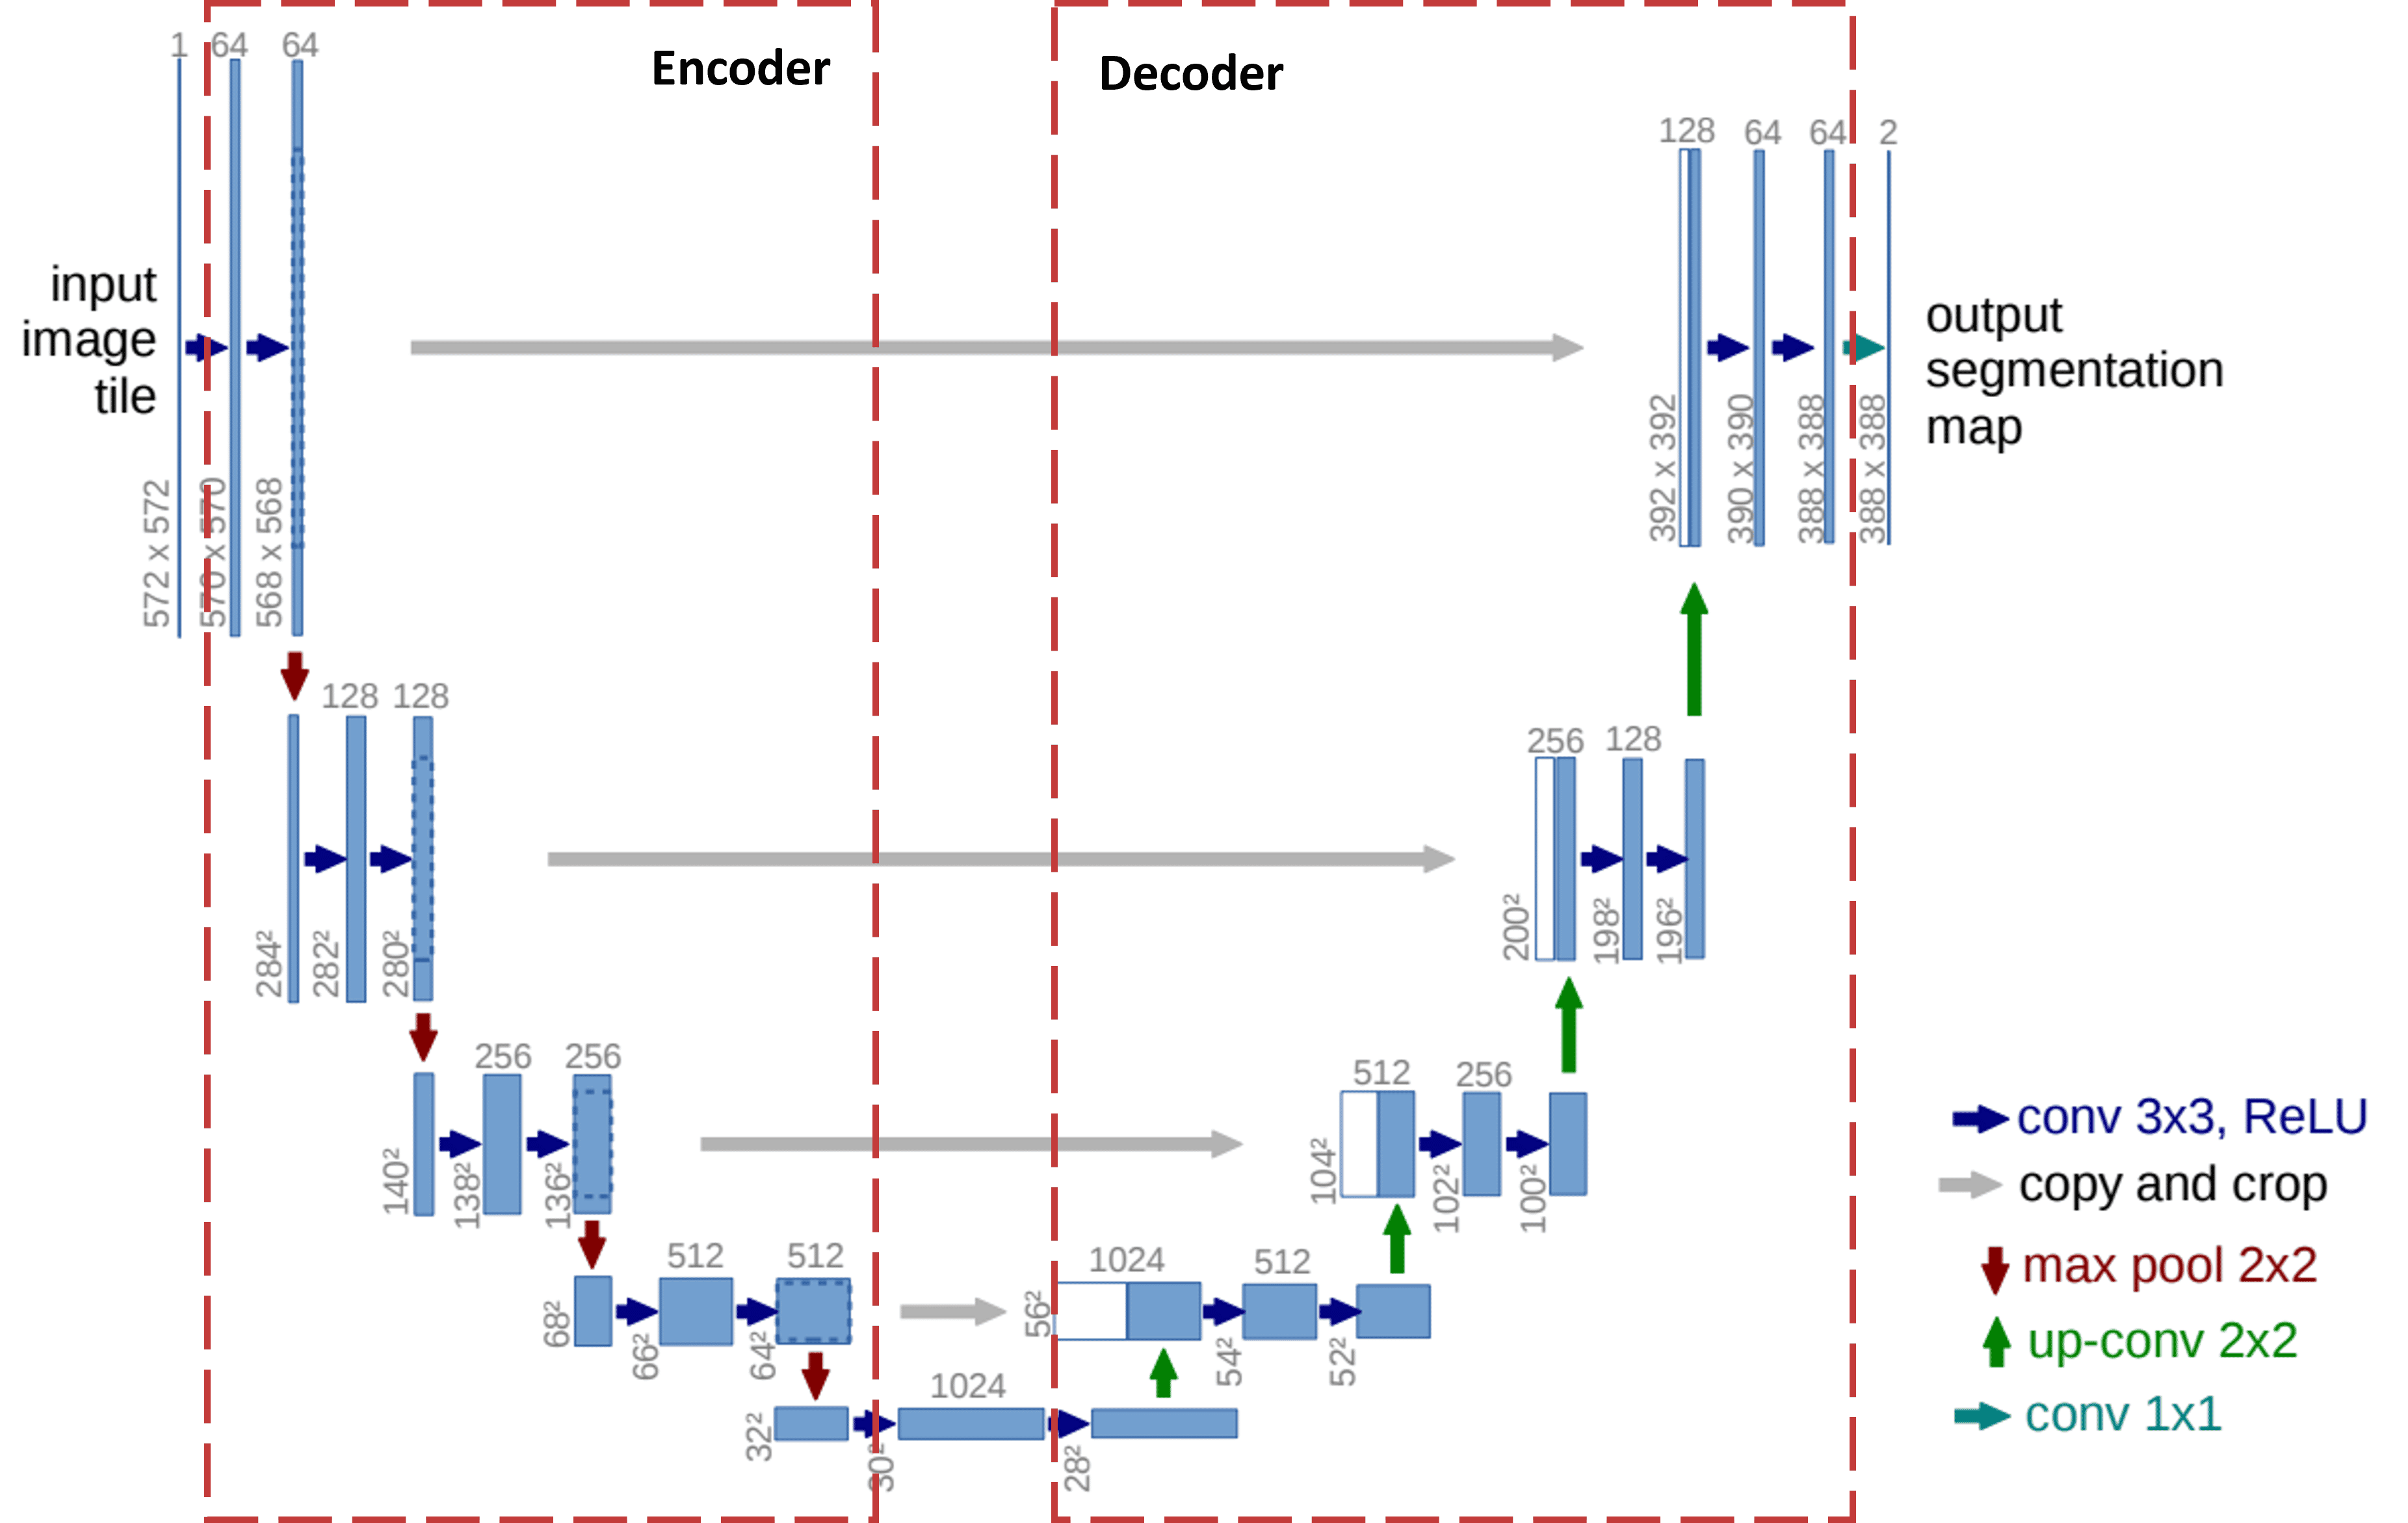
\includegraphics[width=0.88\textwidth]{Figures/Gallery/u-net.png}
    \caption{Kiến trúc U-Net: nhánh encoder giảm mẫu (trái) tăng số kênh đặc trưng, nhánh decoder tăng mẫu (phải) khôi phục độ phân giải không gian. Các mũi tên xám ngang biểu thị skip connections nối đặc trưng tương ứng từ encoder sang decoder.(Nguồn: \cite{Ronneberger2015})}
    \label{fig:unet_arch}
\end{figure}

\subsection{U-Net++}

U-Net++ \cite{Zhou2018} là phần mở rộng của U-Net, giới thiệu các nút trung gian $x^{i,j}$ trên các skip connections, trong đó $i$ là chỉ số độ sâu encoder và $j$ là chỉ số bước trong kiến trúc lồng nhau. Công thức tính nút trung gian:

\begin{equation}
    x^{i,j} = \mathcal{H}\!\left(
        \left[ x^{i,k} \right]_{k=0}^{j-1},\;
        \mathcal{U}(x^{i+1,j-1})
    \right)
    \label{eq:unetpp}
\end{equation}

trong đó $\mathcal{H}$ là khối tích chập dày đặc, $\mathcal{U}$ là phép tăng mẫu, và $[\cdot]$ là phép nối tensor. Mật độ kết nối cao hơn giúp U-Net++ khai thác thông tin đặc trưng ở nhiều tỷ lệ không gian, cải thiện đặc biệt với các cấu trúc có kích thước đa dạng.

Trong hệ thống BrainSeg-XAI, U-Net++ được khởi tạo qua thư viện SMP \cite{Yakubovskiy2019} với encoder EfficientNet-B4 \cite{Tan2019} pretrained trên ImageNet.

\begin{figure}[h!]
    \centering
    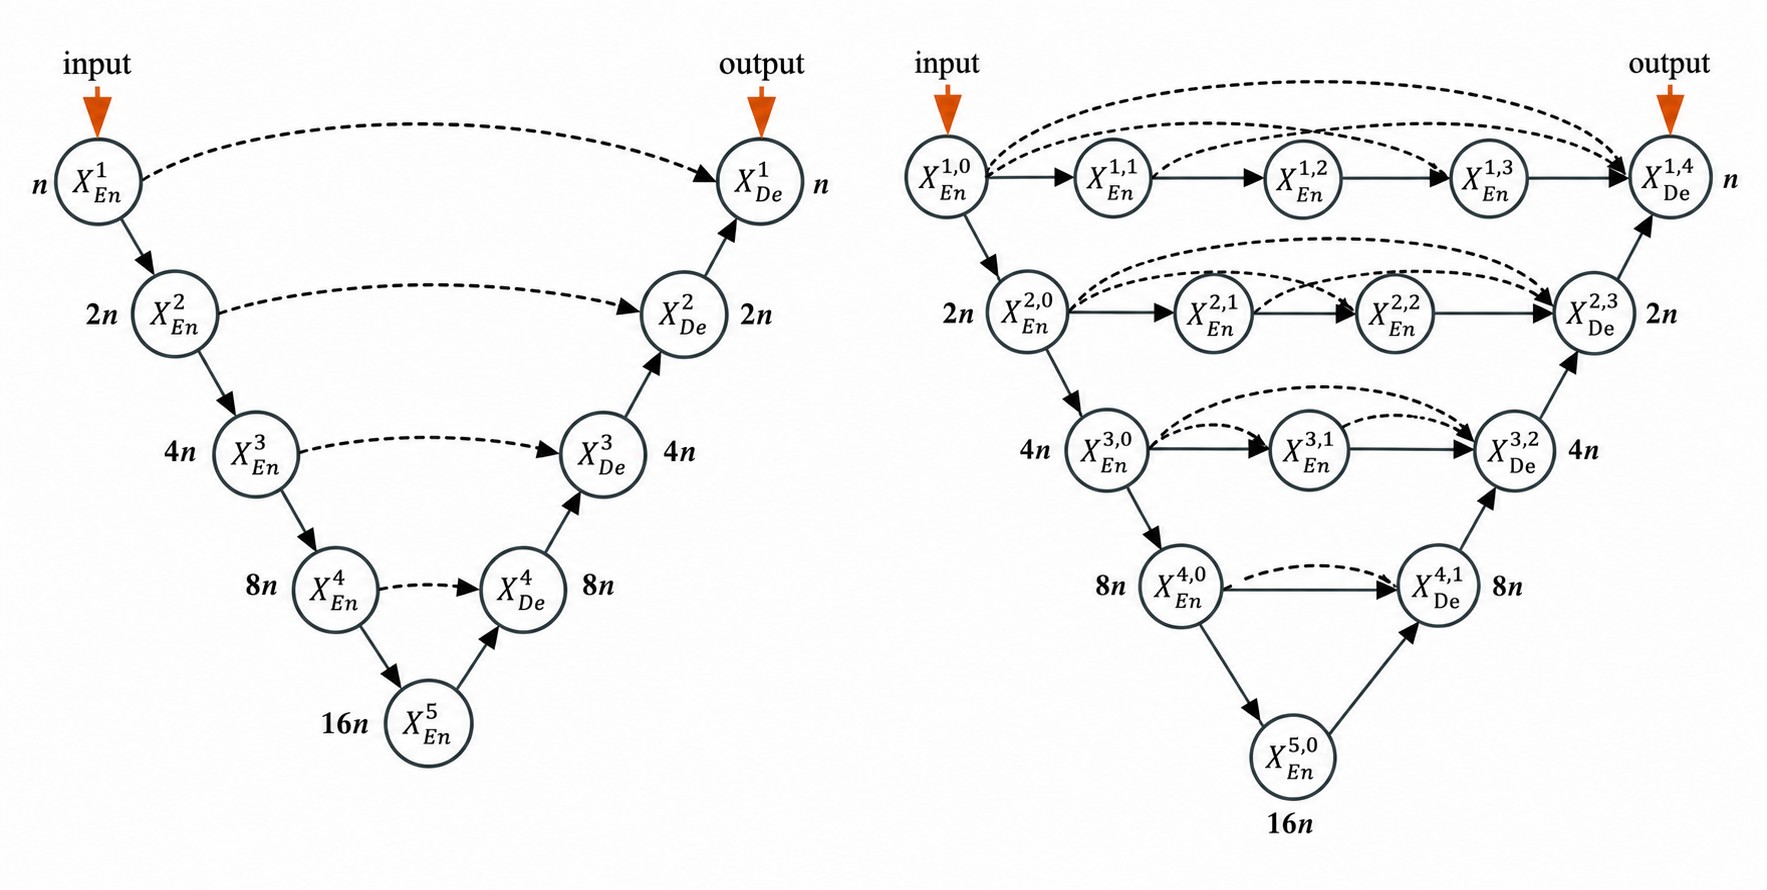
\includegraphics[width=0.82\textwidth]{Figures/Gallery/unet_vs_unetpp.png}
    \caption{So sánh đồ thị kết nối giữa U-Net (trái) và U-Net++ (phải). (Nguồn: \cite{Zhou2018})}
    \label{fig:unetpp_compare}
\end{figure}

\subsection{EfficientNet-B2 làm encoder}

EfficientNet \cite{Tan2019} sử dụng chiến lược ``compound scaling'' -- đồng thời tăng chiều rộng, chiều sâu và độ phân giải theo một hệ số $\phi$ -- để tối ưu hiệu quả tham số. EfficientNet-B2 với khoảng 19 triệu tham số cho hiệu suất cao trên ImageNet trong khi tiêu thụ ít tài nguyên tính toán hơn so với ResNet-50 hay VGG-16. Việc sử dụng encoder pretrained trên ImageNet giúp khởi tạo với các đặc trưng hình ảnh phong phú, quan trọng khi dữ liệu y tế thường hạn chế.

\section{Grad-CAM: Gradient-weighted Class Activation Mapping}

\subsection{Nguyên lý}

Grad-CAM \cite{Selvaraju2017} tính toán tầm quan trọng của mỗi kênh đặc trưng $k$ trong lớp tích chập mục tiêu bằng cách lấy trung bình toàn cục gradient của tín hiệu mục tiêu $y^c$ (đầu ra lớp cuối) theo bản đồ đặc trưng $A^k$:

\begin{equation}
    \alpha_k^c = \frac{1}{Z} \sum_i \sum_j \frac{\partial y^c}{\partial A_{ij}^k}
    \label{eq:gradcam_weight}
\end{equation}

trong đó $Z = H \times W$ là kích thước không gian của bản đồ đặc trưng. Bản đồ Grad-CAM sau đó được tính bằng tổ hợp tuyến tính có trọng số $\alpha_k^c$, áp dụng ReLU để giữ lại chỉ các ảnh hưởng tích cực:

\begin{equation}
    L_{\text{Grad-CAM}}^c = \text{ReLU}\!\left( \sum_k \alpha_k^c A^k \right)
    \label{eq:gradcam_map}
\end{equation}

Kết quả là bản đồ nhiệt có kích thước bằng bản đồ đặc trưng, sau đó được nội suy về kích thước ảnh gốc để trực quan hóa.

\subsection{Triển khai trong BrainSeg-XAI}

Module \texttt{xai/gradcam.py} đăng ký hai hook PyTorch tại thời điểm khởi tạo:
\begin{itemize}
    \item \texttt{register\_forward\_hook}: lưu bản đồ đặc trưng $A^k$ trong lượt truyền xuôi.
    \item \texttt{register\_full\_backward\_hook}: lưu gradient $\partial y^c / \partial A^k$ trong lượt truyền ngược.
\end{itemize}

\begin{sloppypar}
Lớp mục tiêu (\textit{target layer}) được chọn theo loại mô hình: \texttt{model.up4.conv.conv[-3]} cho vanilla UNet (lớp tích chập cuối trước lớp đầu ra); \texttt{model.segmentation\_head[0]} cho SMP (lớp tích chập đầu tiên trong segmentation head).
\end{sloppypar}

Tín hiệu mục tiêu là tổng toàn bộ đầu ra sigmoid: $y^c = \sum_{i,j} \sigma(\text{logit}_{ij})$, phù hợp với bài toán phân đoạn nhị phân nơi không có nhãn lớp đơn.

\section{Hàm mất mát cho phân đoạn nhị phân}

\subsection{Hệ số Dice}

Hệ số Dice đo lường mức độ chồng lấp giữa mặt nạ dự đoán $\hat{Y}$ và nhãn thực $Y$:

\begin{equation}
    \text{Dice}(\hat{Y}, Y) = \frac{2 \sum_{i} \hat{y}_i y_i}{\sum_{i} \hat{y}_i^2 + \sum_{i} y_i^2 + \epsilon}
    \label{eq:dice}
\end{equation}

trong đó $\epsilon$ là hằng số nhỏ để tránh chia cho 0. Hàm mất mát Dice: $\mathcal{L}_{\text{Dice}} = 1 - \text{Dice}$.

\subsection{Binary Cross-Entropy}

Hàm BCE đo lỗi pixel-level:

\begin{equation}
    \mathcal{L}_{\text{BCE}} = -\frac{1}{N} \sum_{i=1}^{N} \left[ y_i \log \hat{p}_i + (1 - y_i) \log(1 - \hat{p}_i) \right]
    \label{eq:bce}
\end{equation}

trong đó $\hat{p}_i = \sigma(\text{logit}_i)$ là xác suất dự đoán pixel $i$ là khối u. Trong thực tế huấn luyện, hàm mất mát kết hợp $\mathcal{L} = \mathcal{L}_{\text{BCE}} + \mathcal{L}_{\text{Dice}}$ thường cho kết quả tốt hơn từng thành phần đơn lẻ.

\section{Trích xuất đặc trưng hình thái học}

\subsection{Phân tích thành phần liên thông}

Hệ thống sử dụng \texttt{scipy.ndimage.label} để phân tách mặt nạ nhị phân thành các thành phần liên thông (connected components). Mỗi thành phần tương ứng với một vùng khối u riêng biệt.

\subsection{Các đặc trưng hình dạng}

\begin{sloppypar}
Trên vùng khối u lớn nhất (largest region), \texttt{skimage.measure.regionprops} cung cấp các thuộc tính sau:
\end{sloppypar}

\textbf{Độ bất đối xứng hình dạng (shape irregularity):}
\begin{equation}
    I_{\text{shape}} = 1 - \frac{4\pi A}{P^2}
    \label{eq:irregularity}
\end{equation}
trong đó $A$ là diện tích (pixel) và $P$ là chu vi. Phần tử $4\pi A / P^2$ chính là chỉ số compactness (nén tròn), bằng 1 khi vùng hoàn toàn hình tròn. Giá trị $I_{\text{shape}}$ cao cho thấy hình dạng bất quy tắc, thường liên quan đến khối u ác tính có ranh giới không đều.

\textbf{Độ phức tạp đường biên (boundary complexity):}
\begin{equation}
    B_c = \frac{P}{\sqrt{A} + \epsilon}
    \label{eq:boundary}
\end{equation}
Tỷ lệ chu vi trên căn bậc hai diện tích phản ánh mức độ gồ ghề của đường biên khối u. Giá trị lớn cho thấy đường biên phức tạp với nhiều lồi lõm.

\textbf{Dịch chuyển đường giữa (midline shift):}
\begin{equation}
    \text{shift} = \left| \frac{c_x}{W} - 0.5 \right| > 0.10
    \label{eq:midline}
\end{equation}
trong đó $c_x$ là tọa độ x tâm khối u và $W$ là chiều rộng ảnh. Dịch chuyển quá 10\% từ đường giữa là chỉ điểm lâm sàng quan trọng về tình trạng hiệu ứng khối.

\textbf{Chuyển đổi đơn vị diện tích:}
Giả sử lát cắt MRI tiêu chuẩn rộng 24 cm trên ảnh $256 \times 256$, hệ số chuyển đổi là $(24/256)^2 \approx 0.00879 \text{ cm}^2/\text{pixel}$.

\section{Hệ thống phân loại cấp độ nguy hiểm (Rule-based Risk Engine)}

\subsection{Thiết kế hệ thống}
Hệ thống cấp độ nguy hiểm được thiết kế theo nguyên lý \textit{additive scoring}: mỗi quy tắc cộng một điểm cố định vào điểm rủi ro tổng hợp $S_{\text{risk}}$, giới hạn tối đa 100. Thiết kế này cho phép truy vết nguyên nhân đóng góp vào điểm rủi ro cuối cùng. Sáu quy tắc hiện có:

\begin{table}[h!]
    \centering
    \caption{Các quy tắc trong bộ máy đánh giá rủi ro y khoa.}
    \label{tab:rules}
    \begin{tabular}{l l r}
        \toprule
        \tabhead{Quy tắc} & \tabhead{Điều kiện} & \tabhead{Điểm cộng} \\
        \midrule
        R1: Tỷ lệ chiếm diện tích   & occupancy $> 20\%$          & $+30$ \\
                                     & occupancy $> 10\%$          & $+20$ \\
                                     & occupancy $> 5\%$           & $+10$ \\
        R2: Bất đối xứng hình dạng  & irregularity $> 0.7$        & $+25$ \\
                                     & irregularity $> 0.5$        & $+15$ \\
        R3: Phức tạp đường biên     & boundary\_complexity $> 15$ & $+20$ \\
                                     & boundary\_complexity $> 10$ & $+10$ \\
        R4: Dịch chuyển đường giữa  & midline\_shift = True       & $+20$ \\
        R5: Số vùng khối u          & num\_regions $> 3$          & $+15$ \\
                                     & num\_regions $> 1$          & $+8$  \\
        R6: Diện tích tuyệt đối     & area $> 10$ cm²             & $+15$ \\
                                     & area $> 4$ cm²              & $+8$  \\
        \bottomrule
    \end{tabular}
\end{table}

\subsection{Phân loại mức rủi ro}

Bốn mức rủi ro được ánh xạ từ điểm số:

\begin{table}[h!]
    \centering
    \caption{Ánh xạ điểm rủi ro sang mức phân loại.}
    \label{tab:risktier}
    \begin{tabular}{l l l l}
        \toprule
        \tabhead{Mức rủi ro} & \tabhead{Khoảng điểm} & \tabhead{Mức độ} & \tabhead{Màu hiển thị} \\
        \midrule
        Thấp       & $0 - 29$  & Nhẹ       & Xanh lá  \\
        Trung bình & $30 - 49$ & Trung bình & Vàng  \\
        Cao        & $50 - 69$ & Nghiêm trọng & Cam  \\
        Rất cao    & $70+$     & Nguy kịch  & Đỏ \\
        \bottomrule
    \end{tabular}
\end{table}

% Chương 3: Phương pháp và kiến trúc hệ thống

\chapter{Phương pháp và kiến trúc hệ thống}

\label{Chapter3}

%----------------------------------------------------------------------------------------

\section{Tổng quan kiến trúc hệ thống}

\begin{figure}[h!]
    \centering
    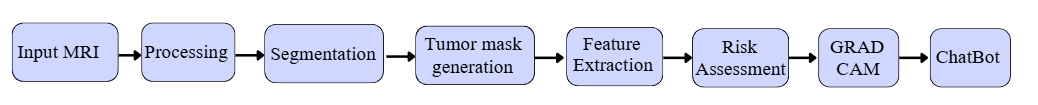
\includegraphics[width=1\textwidth]{Figures/Chapter/Chapter5.png}
    \caption{Pineline phương pháp.}
    \label{fig:pineline}
\end{figure}

%----------------------------------------------------------------------------------------
\subsection*{I. Giai đoạn 1 -- Tiếp nhận và xác thực yêu cầu}
%----------------------------------------------------------------------------------------

\subsection*{1. Endpoint REST}

Endpoint duy nhất cho dự đoán là \texttt{POST /api/v1/predict}, định nghĩa trong \texttt{app/api/predict.py}. FastAPI nhận file qua \texttt{multipart/form-data} nhờ khai báo \texttt{UploadFile = File(...)}.

\subsection*{2. Input MRI}

Trước khi dữ liệu được đưa vào pipeline xử lý chính, hệ thống tiến hành một chuỗi kiểm tra nhằm đảm bảo tính hợp lệ và an toàn của tệp đầu vào. Các bước kiểm tra được thực hiện theo thứ tự như sau:

\begin{sloppypar}
\begin{enumerate}
    \item \textbf{Kiểm tra loại MIME}: Hệ thống xác minh trường \texttt{file.content\_type} phải thuộc nhóm \texttt{"image/"}. Nếu điều kiện không được thỏa mãn, yêu cầu sẽ bị từ chối với mã lỗi HTTP 400.

    \item \textbf{Kiểm tra dung lượng tệp}: Toàn bộ dữ liệu được đọc vào bộ nhớ thông qua lệnh \texttt{raw = await file.read()}. Nếu kích thước vượt quá ngưỡng 20\,MB (\texttt{len(raw) > 20\,MB}), hệ thống trả về mã lỗi HTTP 413 để hạn chế tải tài nguyên.

    \item \textbf{Kiểm tra tính toàn vẹn của ảnh}: Thư viện Pillow được sử dụng để thử mở dữ liệu ảnh. Trong trường hợp tệp bị hỏng hoặc không đúng định dạng, một ngoại lệ sẽ được kích hoạt và hệ thống phản hồi mã lỗi HTTP 422.
\end{enumerate}
\end{sloppypar}
%----------------------------------------------------------------------------------------
\subsection*{II. Giai đoạn 2 -- Tiền xử lý ảnh}
%----------------------------------------------------------------------------------------

\subsection*{1. Chuỗi biến đổi}

Module \texttt{utils/image\_utils.py} thực hiện một chuỗi bốn bước xử lý tuần tự nhằm biến đổi ảnh thô thành định dạng đầu vào phù hợp cho mô hình học sâu.

\begin{sloppypar}
\begin{enumerate}
    \item \textbf{Giải mã và chuẩn hóa không gian màu}: Dữ liệu ảnh được đọc từ byte stream thông qua \texttt{Image.open(BytesIO(raw))} của Pillow. Sau đó, ảnh được chuyển về định dạng RGB để đảm bảo tính nhất quán giữa các trường hợp ảnh đầu vào như grayscale, RGB hoặc RGBA, tất cả đều được đưa về ba kênh màu chuẩn.

    \item \textbf{Thay đổi kích thước ảnh}: Ảnh được resize về kích thước cố định $256 \times 256$ bằng phương pháp nội suy bilinear (\texttt{cv2.INTER\_LINEAR}). Lựa chọn này giúp cân bằng giữa chi phí tính toán và khả năng giữ lại cấu trúc hình ảnh, đặc biệt phù hợp với dữ liệu y tế có biên chuyển tiếp mềm.

    \item \textbf{Chuẩn hóa theo ImageNet}: Giá trị pixel được chuyển sang kiểu float32, chuẩn hóa về khoảng [0,1], sau đó áp dụng chuẩn hóa theo thống kê ImageNet:
    \begin{equation}
        x'_c = \frac{x_c / 255 - \mu_c}{\sigma_c}, \quad
        \boldsymbol{\mu} = [0.485,\,0.456,\,0.406], \quad
        \boldsymbol{\sigma} = [0.229,\,0.224,\,0.225]
        \label{eq:imagenet_norm}
    \end{equation}
    Việc sử dụng chuẩn hóa này nhằm đảm bảo đầu vào phù hợp với phân phối dữ liệu mà encoder EfficientNet-B4 đã được huấn luyện trước, giúp giảm hiện tượng lệch phân phối và cải thiện độ ổn định khi suy luận.

    \item \textbf{Chuyển đổi tensor và bổ sung batch dimension}: Ảnh sau khi chuẩn hóa được chuyển từ định dạng HWC sang CHW bằng \texttt{np.transpose}, sau đó chuyển thành \texttt{torch.FloatTensor}. Cuối cùng, một chiều batch được thêm vào bằng \texttt{.unsqueeze(0)}, tạo tensor đầu vào có kích thước $[1, 3, 256, 256]$.
\end{enumerate}
\end{sloppypar}

\subsection*{2. Xử lý đầu ra để trực quan hóa}

Sau suy luận, mặt nạ nhị phân $\hat{M} \in \{0,1\}^{256\times256}$ được trực quan hóa bằng cách overlay: pixel khối u (\texttt{mask=1}) được tô màu xanh lá \texttt{RGB = [0, 255, 136]}, giúp phân biệt rõ với mô não xung quanh. Kết quả được mã hóa PNG qua \texttt{BytesIO} và chuyển sang base64 string.

%----------------------------------------------------------------------------------------
\subsection*{III. Giai đoạn 3 -- Tải và nhận dạng mô hình}
%----------------------------------------------------------------------------------------

\subsection*{1. Cơ chế lazy loading}

Module \texttt{services/inference.py} khai báo ba biến module-level: \texttt{\_model = None}, \texttt{\_model\_type = None}, \texttt{\_gradcam = None}. Hàm \texttt{\_load\_model()} chỉ thực thi khi một trong ba biến này còn là \texttt{None}, tức là chỉ xảy ra một lần duy nhất trong suốt vòng đời server. Chiến lược này:

\begin{itemize}
    \item Giảm thời gian khởi động server (không tải PyTorch model khi import module).
    \item Tránh chiếm VRAM/RAM GPU cho đến khi có request thực sự.
    \item Thread-safe với GIL của Python trong môi trường single-worker.
\end{itemize}

\subsection*{2. Tự động nhận dạng loại checkpoint}

File \texttt{unet\_best.pth} có thể chứa hai loại kiến trúc khác nhau. Hệ thống phân biệt qua tên khóa trong \texttt{state\_dict}:

\begin{sloppypar}
\begin{itemize}
    \item \textbf{Vanilla UNet}: Các khóa bắt đầu bằng \texttt{inc.}, \texttt{down1.}, \ldots, \texttt{up4.}, \texttt{outc.} -- do lớp Python \texttt{UNet} định nghĩa trực tiếp trong \texttt{models/unet.py}.
    \item \textbf{SMP model}: Các khóa theo cấu trúc SMP như \texttt{encoder.*}, \texttt{decoder.*}, \texttt{segmentation\_head.*}. Kèm theo, checkpoint lưu thêm trường \texttt{arch} (e.g. \texttt{"unetplusplus"}) và \texttt{encoder} (e.g. \texttt{"efficientnet-b4"}) ở cấp từ điển ngoài.
\end{itemize}
\end{sloppypar}

\begin{sloppypar}
Sau khi nhận dạng, hệ thống tạo đúng instance model, tải trọng số, gọi \texttt{model.eval()} và chuyển sang \texttt{DEVICE} (CUDA nếu có, ngược lại CPU). Chi tiết mã nguồn tại Phụ lục~\ref{AppendixA}.
\end{sloppypar}

%----------------------------------------------------------------------------------------
\subsection*{IV. Giai đoạn 4 -- Suy luận mô hình}
%----------------------------------------------------------------------------------------

\subsection*{1. Forward pass và tạo mặt nạ}

Sau khi tensor đầu vào $\mathbf{x} \in \mathbb{R}^{1 \times 3 \times 256 \times 256}$ được đưa lên đúng \texttt{DEVICE}, suy luận diễn ra trong ba bước:

\begin{sloppypar}
\begin{enumerate}
    \item \textbf{Forward pass không gradient}: Sử dụng \texttt{torch.no\_grad()} để tắt việc duy trì đồ thị tính toán, tiết kiệm bộ nhớ trong giai đoạn suy luận thuần:
    \[ \text{logits} = f_\theta(\mathbf{x}), \quad \text{logits} \in \mathbb{R}^{1 \times 1 \times 256 \times 256} \]
    \item \textbf{Áp dụng sigmoid và ngưỡng}: Chuyển logits sang xác suất rồi nhị phân hóa:
    \begin{equation}
        \hat{M}_{ij} = \begin{cases} 1 & \text{nếu } \sigma(\text{logit}_{ij}) > 0.5 \\ 0 & \text{ngược lại} \end{cases}
        \label{eq:threshold}
    \end{equation}
    \item \textbf{Chuyển về ndarray}: \texttt{.squeeze().cpu().numpy().astype(np.uint8)} tạo mảng $256\times256$ với giá trị 0/1.
\end{enumerate}
\end{sloppypar}

\subsection*{2. Lý do chọn ngưỡng 0.5}

Ngưỡng 0.5 là giá trị trung tính mặc định của sigmoid. Trong thực tế, ngưỡng tối ưu có thể được điều chỉnh dựa trên đường cong ROC để cân bằng Precision/Recall theo yêu cầu lâm sàng (ưu tiên Recall cao hơn để giảm FN). Tuy nhiên, giá trị 0.5 được giữ nguyên để đảm bảo tính nhất quán và tái sản xuất kết quả.

%----------------------------------------------------------------------------------------
\subsection*{V. Giai đoạn 5 -- Tạo bản đồ Grad-CAM}
%----------------------------------------------------------------------------------------

\subsection*{1. Đăng ký hooks}

Lớp \texttt{GradCAM} trong \texttt{xai/gradcam.py} đăng ký hai hook PyTorch ngay khi khởi tạo -- không phải mỗi lần gọi. Điều này tránh tích lũy hooks gây rò rỉ bộ nhớ và overhead:

\begin{sloppypar}
\begin{itemize}
    \item \texttt{register\_forward\_hook} trên \texttt{target\_layer}: Lưu bản đồ đặc trưng $\{A^k\}_{k=1}^{K}$ sau lượt forward.
    \item \texttt{register\_full\_backward\_hook} trên \texttt{target\_layer}: Lưu gradient $\{\partial y^c / \partial A^k\}$ sau lượt backward.
\end{itemize}
\end{sloppypar}

Lớp mục tiêu được chọn theo loại mô hình:
\begin{itemize}
    \item Vanilla UNet: \texttt{model.up4.conv.conv[-3]} -- lớp tích chập cuối cùng trước lớp đầu ra, giàu đặc trưng không gian cao nhất.
    \item SMP: \texttt{model.segmentation\_head[0]} -- lớp tích chập đầu tiên trong segmentation head, là điểm hội tụ của toàn bộ thông tin decoder.
\end{itemize}

\subsection*{2. Quy trình tạo bản đồ}

Grad-CAM chạy theo quy trình tám bước cho mỗi ảnh:

\begin{enumerate}
    \item Tách tensor khỏi đồ thị (detach), bật \texttt{requires\_grad = True} để cho phép backward.
    \item Forward pass: hooks lưu $\{A^k\}$.
    \item Tính tín hiệu mục tiêu: $y^c = \sum_{i,j} \sigma(\text{output}_{ij})$ -- tổng xác suất sigmoid toàn ảnh, phù hợp với bài toán phân đoạn không có nhãn lớp đơn.
    \item Backward pass: hooks lưu $\{\partial y^c / \partial A^k\}$.
    \item Tính trọng số Global Average Pooling: $\alpha_k = \frac{1}{HW}\sum_{i,j} \frac{\partial y^c}{\partial A^k_{ij}}$.
    \item Tổng hợp bản đồ thô: $L = \text{ReLU}\!\left(\sum_k \alpha_k A^k\right)$.
    \item Nội suy bilinear về $256\times256$.
    \item Chuẩn hóa min-max về $[0, 1]$, ánh xạ sang JET colormap (OpenCV), blend 50/50 với ảnh gốc bằng \texttt{cv2.addWeighted}.
\end{enumerate}

Bước ReLU tại bước 6 loại bỏ các ảnh hưởng âm -- những vùng \textit{ức chế} quyết định phân đoạn -- chỉ giữ lại các vùng \textit{kích hoạt} tích cực, làm cho heatmap dễ diễn giải hơn về mặt lâm sàng.

%----------------------------------------------------------------------------------------
\subsection*{VI. Giai đoạn 6 -- Trích xuất đặc trưng hình thái}
%----------------------------------------------------------------------------------------

\subsection*{1. Phân tích thành phần liên thông}

Module \texttt{services/feature\_extraction.py} nhận mặt nạ nhị phân $\hat{M}$ và trích xuất vector đặc trưng hình thái. Bước đầu tiên dùng \texttt{scipy.ndimage.label} để phân tách mask thành các thành phần liên thông (connected components), từ đó đếm \texttt{num\_regions} -- số vùng khối u riêng biệt phát hiện được. Đây là chỉ số quan trọng: $\texttt{num\_regions} > 1$ gợi ý khối u đa ổ.

\subsection*{2.Tính toán thuộc tính vùng}

\begin{sloppypar}
Trên vùng khối u lớn nhất (largest component), \texttt{skimage.measure.regionprops} cung cấp:
\end{sloppypar}
\begin{itemize}
    \item \texttt{area}: Số pixel dương tính.
    \item \texttt{perimeter}: Chu vi tính bằng xấp xỉ bề mặt (4-connectivity).
    \item \texttt{centroid}: Tọa độ $(c_x, c_y)$ tâm hình học.
\end{itemize}

Từ ba giá trị này, năm đặc trưng dẫn xuất được tính theo các công thức tại Chương~\ref{Chapter2} (phương trình \ref{eq:irregularity}--\ref{eq:midline}):

\begin{table}[h!]
    \centering
    \caption{Các đặc trưng hình thái học trích xuất từ mặt nạ phân đoạn.}
    \label{tab:features_pipeline}
    \begin{tabular}{l l l}
        \toprule
        \tabhead{Đặc trưng} & \tabhead{Công thức} & \tabhead{Ý nghĩa lâm sàng} \\
        \midrule
        \texttt{occupancy\_ratio}     & $A_\text{px} / 256^2 \times 100$     & Tỷ lệ chiếm não (\%) \\
        \texttt{shape\_irregularity}  & $1 - 4\pi A / P^2$                   & Độ bất quy tắc hình dạng \\
        \texttt{boundary\_complexity} & $P / \sqrt{A}$                       & Độ gồ ghề đường biên \\
        \texttt{midline\_shift}       & $|c_x/256 - 0.5| > 0.10$            & Dịch chuyển đường giữa \\
        \texttt{tumor\_area\_px2} & $S_{tumor\_pixels}$ & Diện tích khối u (px$^2$) \\
        \bottomrule
    \end{tabular}
\end{table}

\subsection*{3. Xác định vị trí giải phẫu}

Tọa độ tâm chuẩn hóa $(\hat{c}_x, \hat{c}_y) = (c_x/256, c_y/256)$ được ánh xạ sang vị trí giải phẫu xấp xỉ:
\begin{itemize}
    \item Theo trục dọc: $\hat{c}_y < 0.33$ → thùy trán; $0.33 \leq \hat{c}_y < 0.67$ → thùy đỉnh/thái dương; $\hat{c}_y \geq 0.67$ → thùy chẩm/tiểu não.
    \item Theo trục ngang: $\hat{c}_x < 0.45$ → bán cầu trái; $\hat{c}_x > 0.55$ → bán cầu phải; còn lại → trung tâm.
\end{itemize}

%----------------------------------------------------------------------------------------
\subsection*{VII. Giai đoạn 7 -- Đánh giá rủi ro lâm sàng}
%----------------------------------------------------------------------------------------

\subsection*{1.Hệ thống phân loại cấp độ nguy hiểm}

\begin{sloppypar}
Module \texttt{rules/medical\_rules.py} triển khai bộ máy đánh giá rủi ro theo nguyên tắc \textit{additive scoring}: mỗi trong sáu quy tắc độc lập kiểm tra một đặc trưng hình thái và cộng điểm vào biến tích lũy \texttt{score}, được giới hạn ở 100. Thiết kế này đảm bảo:
\begin{itemize}
    \item \textbf{Tính giải thích được}: Mỗi quy tắc kích hoạt đều ghi nhận thông báo mô tả cụ thể (ví dụ: \textit{``Tỷ lệ chiếm vùng não rất cao: 31.87\% > 20\%''}).
    \item \textbf{Tính kiểm tra được}: Bộ máy không phải black-box -- mỗi quyết định có thể truy vết nguồn gốc.
    \item \textbf{Khả năng bảo trì}: Thêm, bớt hoặc điều chỉnh ngưỡng của một quy tắc không ảnh hưởng đến các quy tắc còn lại.
\end{itemize}
\end{sloppypar}

\subsection*{2. Kết quả đánh giá}

\begin{sloppypar}
Hàm \texttt{evaluate\_risk(features)} trả về dataclass \texttt{RuleResult} gồm: \texttt{risk\_score}, \texttt{risk\_level} (Thấp/Trung bình/Cao/Rất cao), \texttt{severity}, \texttt{risk\_color} (mã hex), \texttt{fired\_rules} (list quy tắc kích hoạt), \texttt{recommendations} (list khuyến nghị) và \texttt{explanation} (tóm tắt nguyên nhân).
\end{sloppypar}

%----------------------------------------------------------------------------------------
\subsection*{VIII. Giai đoạn 8 -- Xây dựng phản hồi và giao diện người dùng}
%----------------------------------------------------------------------------------------

\subsection*{1. Đóng gói JSON response}

Sau khi hoàn thành các giai đoạn 1--7, hàm \texttt{predict()} trong \texttt{services/inference.py} đóng gói kết quả thành từ điển Python, FastAPI tự động serialize sang JSON:

\begin{itemize}
    \item \textbf{5 ảnh base64}: \texttt{original}, \texttt{mask}, \texttt{overlay}, \texttt{heatmap}, \texttt{cam\_overlay} -- mỗi ảnh là chuỗi base64 của PNG được mã hóa qua \texttt{BytesIO}.
    \item \textbf{features}: Toàn bộ 12 trường đặc trưng hình thái (kể cả \texttt{tumor\_detected}, \texttt{location}, \texttt{centroid\_x/y}).
    \item \textbf{risk}: Cấu trúc \texttt{RuleResult} với điểm, mức, màu, quy tắc kích hoạt và khuyến nghị.
\end{itemize}

\subsection*{2. Kiến trúc frontend React}

Frontend tại \texttt{frontend/src/} nhận JSON và phân phối vào ba thành phần chính:

\begin{sloppypar}
\begin{itemize}
    \item \texttt{App.js}: Điều phối upload $\to$ gọi \texttt{api.predict(formData)} $\to$ cập nhật state \texttt{\{images, features, risk\}}.
    \item \texttt{ImageViewer.jsx}: Hiển thị năm ảnh base64 qua thẻ \texttt{<img>} (data URI base64 PNG), cho phép chuyển đổi qua tab (original / mask / overlay / heatmap / cam\_overlay).
    \item \texttt{RiskPanel.jsx}: Vẽ đồng hồ SVG arc gauge với góc quay tỷ lệ với \texttt{risk\_score}, đổi màu theo \texttt{risk\_color}, liệt kê \texttt{fired\_rules} và \texttt{recommendations}.
\end{itemize}
\end{sloppypar}

\section{Hàm mất mát cho phân đoạn nhị phân}

\subsection{Hệ số Dice}

Hệ số Dice đo lường mức độ chồng lấp giữa mặt nạ dự đoán $\hat{Y}$ và nhãn thực $Y$:

\begin{equation}
    \text{Dice}(\hat{Y}, Y) = \frac{2 \sum_{i} \hat{y}_i y_i}{\sum_{i} \hat{y}_i^2 + \sum_{i} y_i^2 + \epsilon}
    \label{eq:dice}
\end{equation}

trong đó $\epsilon$ là hằng số nhỏ để tránh chia cho 0. Hàm mất mát Dice: $\mathcal{L}_{\text{Dice}} = 1 - \text{Dice}$.

\subsection{Binary Cross-Entropy}

Hàm BCE đo lỗi pixel-level:

\begin{equation}
    \mathcal{L}_{\text{BCE}} = -\frac{1}{N} \sum_{i=1}^{N} \left[ y_i \log \hat{p}_i + (1 - y_i) \log(1 - \hat{p}_i) \right]
    \label{eq:bce}
\end{equation}

trong đó $\hat{p}_i = \sigma(\text{logit}_i)$ là xác suất dự đoán pixel $i$ là khối u. Trong thực tế huấn luyện, hàm mất mát kết hợp $\mathcal{L} = \mathcal{L}_{\text{BCE}} + \mathcal{L}_{\text{Dice}}$ thường cho kết quả tốt hơn từng thành phần đơn lẻ.


\section{Bộ dữ liệu LGG MRI Segmentation}

\subsection{Mô tả tập dữ liệu}

Bộ dữ liệu LGG MRI Segmentation \cite{Buda2019, Buda2019Journal} do Buda và cộng sự phát triển và công bố công khai trên Kaggle. Dữ liệu được lấy từ The Cancer Genome Atlas (TCGA) và bao gồm:

\begin{itemize}
    \item \textbf{Tổng số ảnh:} 3.929 ảnh MRI não 2D (lát cắt axial).
    \item \textbf{Số bệnh nhân:} 110 bệnh nhân được chẩn đoán u thần kinh đệm độ thấp (LGG).
    \item \textbf{Định dạng:} TIFF ($256 \times 256$ pixel, 3 kênh RGB).
    \item \textbf{Nhãn:} Mặt nạ phân đoạn nhị phân ($256 \times 256$) do chuyên gia chú thích, giá trị 255 tương ứng vùng khối u.
    \item \textbf{Chuỗi xung:} Chủ yếu T1-weighted post-contrast.
    \item \textbf{Đặc điểm phân bố:} Phần lớn ảnh không có khối u hoặc khối u nhỏ, tạo ra sự mất cân bằng lớp đáng kể (khoảng 80\% ảnh có tỷ lệ pixel khối u $< 5\%$).
\end{itemize}

\subsection{Chia tập dữ liệu}

Dữ liệu được chia theo bệnh nhân (patient-level split) để tránh rò rỉ thông tin giữa tập train và test:

\begin{table}[h!]
    \centering
    \caption{Phân chia tập dữ liệu LGG MRI Segmentation.}
    \label{tab:dataset_split}
    \begin{tabular}{l r r r}
        \toprule
        \tabhead{Tập dữ liệu} & \tabhead{Số ảnh} & \tabhead{Tỷ lệ} \\
        \midrule
        Train     &  3.143  & 80\% \\
        Val       &  590    & 15\% \\
        Test       & 196    & 5\% \\
        \midrule
        Tổng cộng   & 3.929            & 100\% \\
        \bottomrule
    \end{tabular}
\end{table}

\section{Quy trình huấn luyện}

\subsection{Tăng cường dữ liệu}

Để giảm overfitting và cải thiện khả năng tổng quát hóa \cite{Shorten2019}, các phép biến đổi tăng cường dữ liệu ngẫu nhiên được áp dụng trong quá trình huấn luyện:

\begin{itemize}
    \item Lật ngang (horizontal flip) với xác suất 50\%.
    \item Lật dọc (vertical flip) với xác suất 50\%.
    \item Xoay ngẫu nhiên trong khoảng $\pm 20°$.
    \item Biến đổi độ sáng/tương phản ngẫu nhiên ($\pm 20\%$).
    \item Dịch chuyển ngẫu nhiên theo chiều ngang/dọc (shift range $10\%$).
\end{itemize}

Các phép biến đổi được áp dụng đồng thời cho cả ảnh và nhãn để đảm bảo tính nhất quán.

\subsection{Cấu hình huấn luyện}

\begin{table}[h!]
    \centering
    \caption{Siêu tham số huấn luyện mô hình.}
    \label{tab:hyperparams}
    \begin{tabular}{l l}
        \toprule
        \tabhead{Siêu tham số} & \tabhead{Giá trị} \\
        \midrule
        Optimizer              & Adam \\
        Learning rate ban đầu  & $1 \times 10^{-4}$ \\
        Weight decay           & $1 \times 10^{-5}$ \\
        Batch size             & 16 \\
        Số epoch tối đa        & 50 \\
        Hàm mất mát            & BCE + Dice Loss \\
        Early stopping         & Patience = 10 epoch \\
        LR scheduler           & ReduceLROnPlateau (factor=0.5) \\
        Kích thước ảnh đầu vào & $256 \times 256$ \\
        \bottomrule
    \end{tabular}
\end{table}

\subsection{Môi trường thực nghiệm}

Huấn luyện được thực hiện trên Google Colab Pro với GPU NVIDIA Tesla T4 (16 GB VRAM). Framework sử dụng PyTorch \cite{Paszke2019} v2.0+ và thư viện SMP \cite{Yakubovskiy2019} v0.3+.

\section{Các độ đo đánh giá}

\subsection{Hệ số Dice (DSC)}

Hệ số Dice (Dice Similarity Coefficient) là độ đo chính cho bài toán phân đoạn y tế:

\begin{equation}
    \text{DSC} = \frac{2 \cdot |\hat{Y} \cap Y|}{|\hat{Y}| + |Y|}
    \label{eq:dsc}
\end{equation}

DSC = 1.0 là hoàn hảo; DSC = 0.0 là không chồng lấp. DSC đặc biệt phù hợp với dữ liệu mất cân bằng lớp vì tập trung vào vùng dương tính.

\subsection{Intersection over Union (IoU)}

IoU (Jaccard Index) đo tỷ lệ vùng chồng lấp trên vùng hợp:

\begin{equation}
    \text{IoU} = \frac{|\hat{Y} \cap Y|}{|\hat{Y} \cup Y|} = \frac{\text{TP}}{\text{TP} + \text{FP} + \text{FN}}
    \label{eq:iou}
\end{equation}

\subsection{Precision và Recall}

\begin{equation}
    P = \frac{\text{TP}}{\text{TP} + \text{FP}}, \qquad
    R = \frac{\text{TP}}{\text{TP} + \text{FN}}
    \label{eq:pr}
\end{equation}

\begin{equation}
\text{F1-score} = 2 \cdot \frac{\text{Precision} \cdot \text{Recall}}{\text{Precision} + \text{Recall}}
\end{equation}

Trong bài toán phát hiện u não, Recall (độ phủ) quan trọng hơn Precision: bỏ sót khối u (FN cao) là lỗi nghiêm trọng hơn báo dương giả (FP cao).

% Chương 4: Kết quả thực nghiệm

\chapter{Kết quả thực nghiệm}

\label{Chapter4}

%----------------------------------------------------------------------------------------

\section{Kết quả phân đoạn -- Benchmark 4 mô hình}

\subsection{Thiết lập thực nghiệm}

Bốn kiến trúc được huấn luyện và đánh giá độc lập trên cùng bộ dữ liệu LGG, sử dụng thư viện SMP \cite{Yakubovskiy2019} với encoder pretrained trên ImageNet. Để tối ưu ngưỡng phân loại, mỗi mô hình thực hiện grid search trên tập validation, sau đó áp dụng Test-Time Augmentation (TTA) khi đánh giá cuối. Bảng~\ref{tab:model_configs} tóm tắt cấu hình riêng của từng mô hình:

\begin{table}[h!]
    \centering
    \caption{Cấu hình thực nghiệm của bốn mô hình được đánh giá.}
    \label{tab:model_configs}
    \resizebox{\textwidth}{!}{%
    \begin{tabular}{l l r r r l}
        \toprule
        \tabhead{Mô hình} & \tabhead{Encoder} & \tabhead{Kích thước ảnh} & \tabhead{Epochs} & \tabhead{Ngưỡng} \\
        \midrule
        U-Net (SMP)   &  & $256\times256$ & 36 & 0.725 \\
        U-Net (SMP)   & ResNet-50       & $384\times384$ & 45 & 0.730  \\
        U-Net++ (SMP) & EfficientNet-B2 & $256\times256$ & 62 & 0.500 \\
        ResUNet (SMP) & ResNet-34       & $256\times256$ & 60 & 0.450 \\
        \bottomrule
    \end{tabular}}
\end{table}

\subsection{Bảng benchmark so sánh}

\begin{table}[h!]
    \centering
    \caption{Kết quả thực nghiệm.}
    \label{tab:benchmark}
    \resizebox{\textwidth}{!}{%
    \begin{tabular}{l l r r r r r}
        \toprule
        Kiến trúc & Encoder & Dice & IoU & Precision & Recall & F1-Score \\
        \midrule
        U-Net (SMP)   & -                & 0.7794 & 0.6385 & 0.8666 & 0.7081 & 0.7760 \\
        U-Net (SMP)   & ResNet-50       & 0.7766 & 0.6348 & 0.8396 & 0.7225 & 0.7780 \\
        U-Net++ (SMP) & EfficientNet-B2 & 0.7992 & 0.6656 & 0.8946 & 0.7220 & 0.7766 \\
        \textbf{ResUNet (SMP)} & \textbf{ResNet-34} & \textbf{0.8846} & \textbf{0.7931} & \textbf{0.8929} & \textbf{0.8764} & \textbf{0.8846} \\
        \bottomrule
    \end{tabular}}
\end{table}

\textbf{ResUNet + ResNet-34 vượt trội hoàn toàn} so với ba kiến trúc còn lại trên mọi độ đo:  DiCe 0.8846 cao hơn U-Net tới $+10.5\%$ ; IoU 0.7931 cao hơn U-net $+15.5\%$; Recall 0.8764 cho thấy tỷ lệ bỏ sót khối u rất thấp. Đây là kết quả đáng chú ý vì ResNet-34 là encoder nhẹ nhưng kiến trúc ResUNet tận dụng residual connections để học đặc trưng biên sắc nét hơn.

\subsection{Lịch sử huấn luyện}

\begin{figure}[htbp]
    \centering
    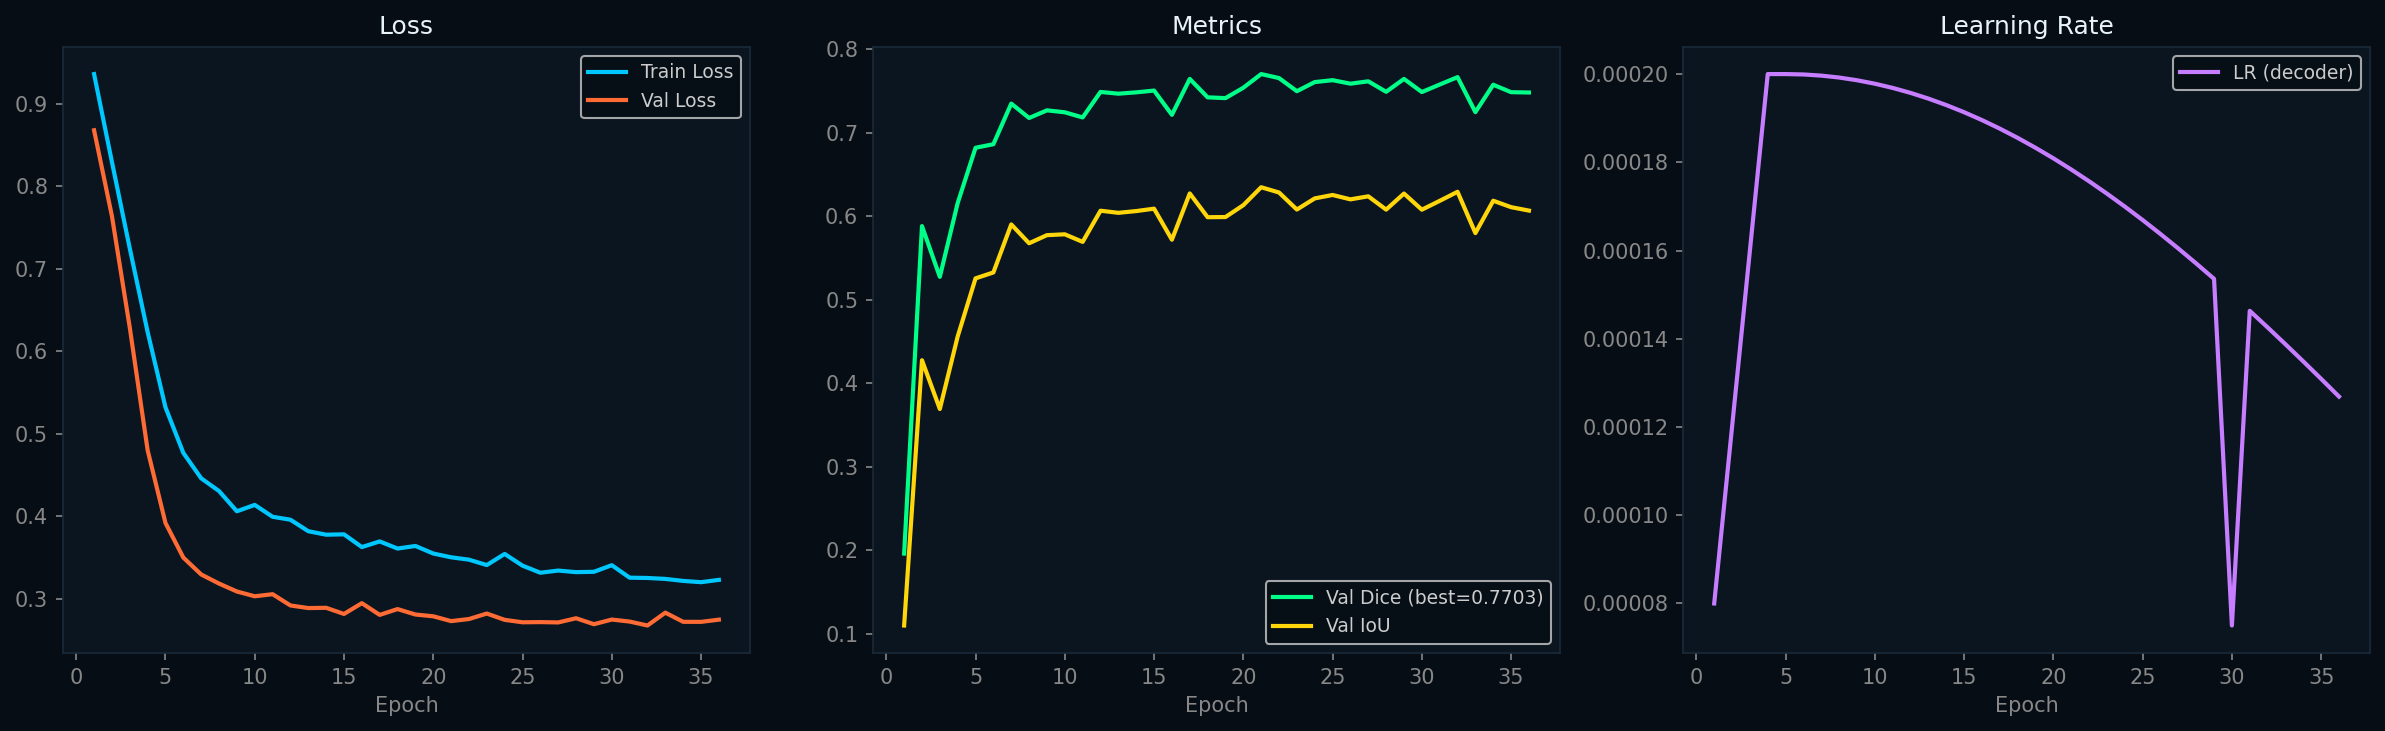
\includegraphics[width=\textwidth]{Figures/Gallery/m1_uneteffb2_history.png}
    \caption{Lịch sử huấn luyện U-Net (EfficientNet-B2).}
    \label{fig:hist_unet_effb2}
\end{figure}

\begin{figure}[htbp]
    \centering
    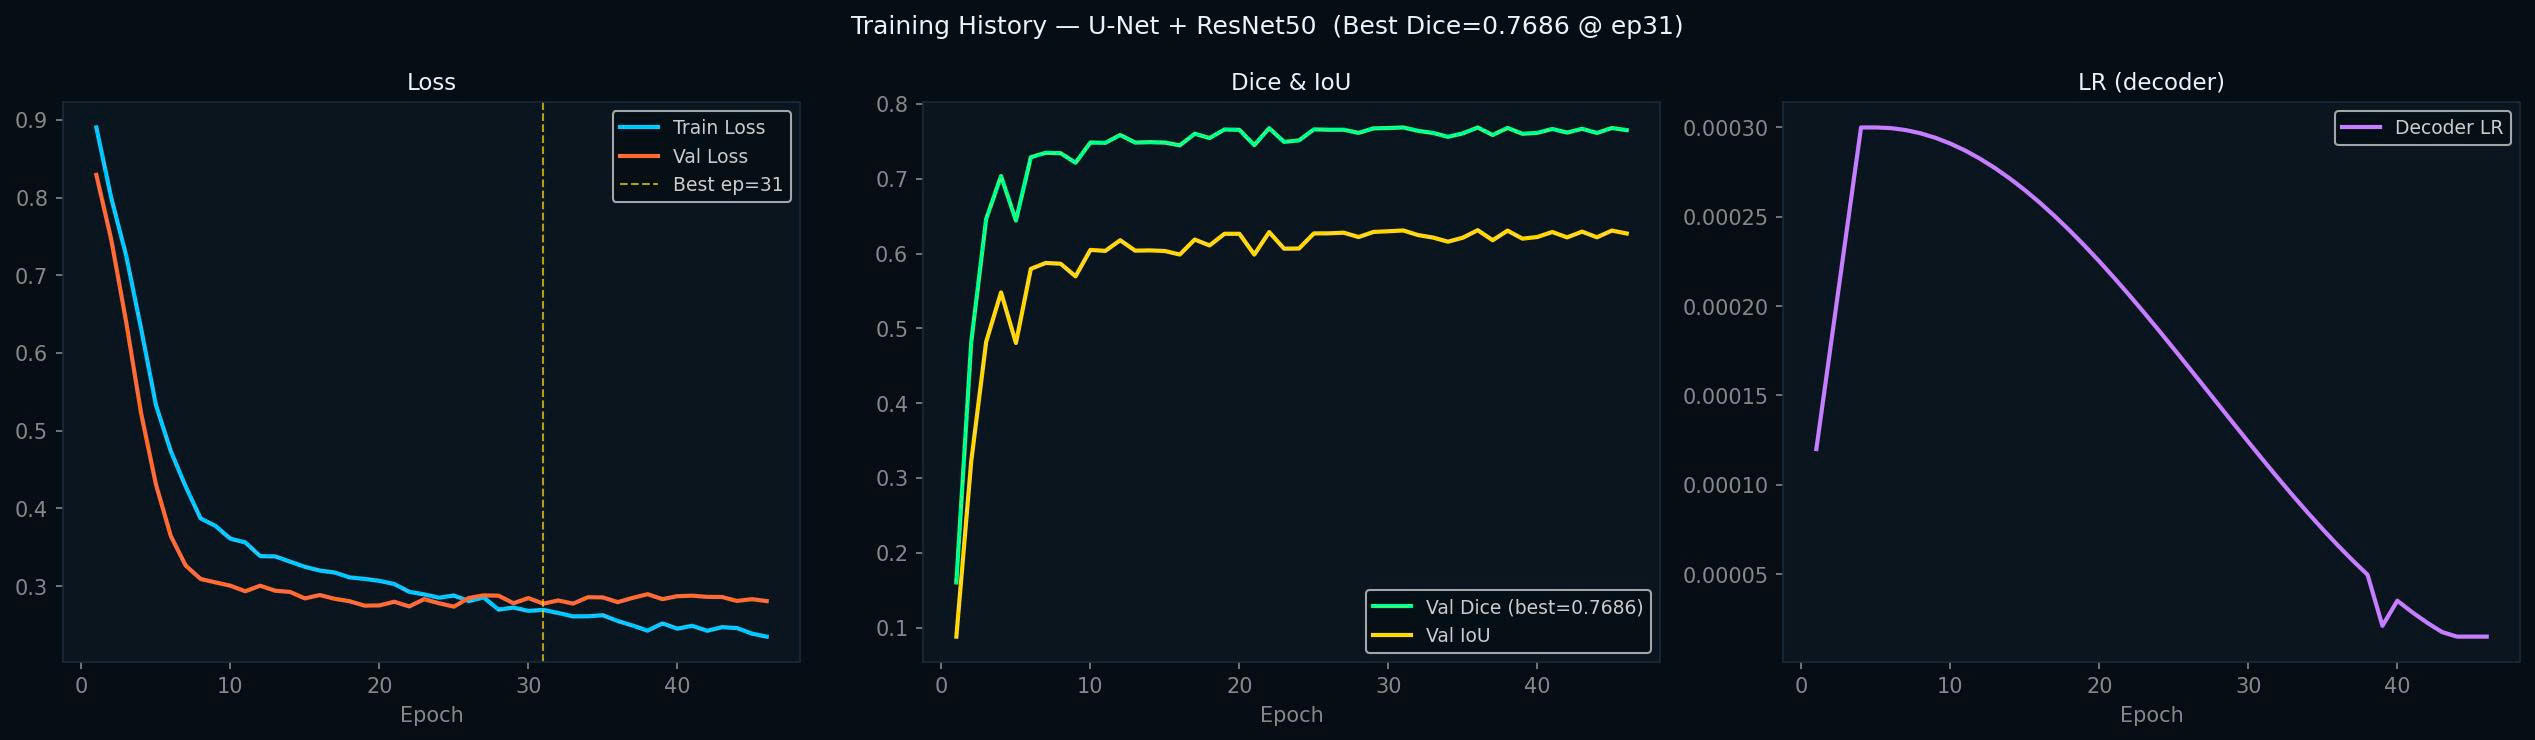
\includegraphics[width=\textwidth]{Figures/Gallery/m2_unetresnet50_history.jpg}
    \caption{Lịch sử huấn luyện U-Net (ResNet-50).}
    \label{fig:hist_unet_resnet50}
\end{figure}

\FloatBarrier

\begin{figure}[htbp]
    \centering
    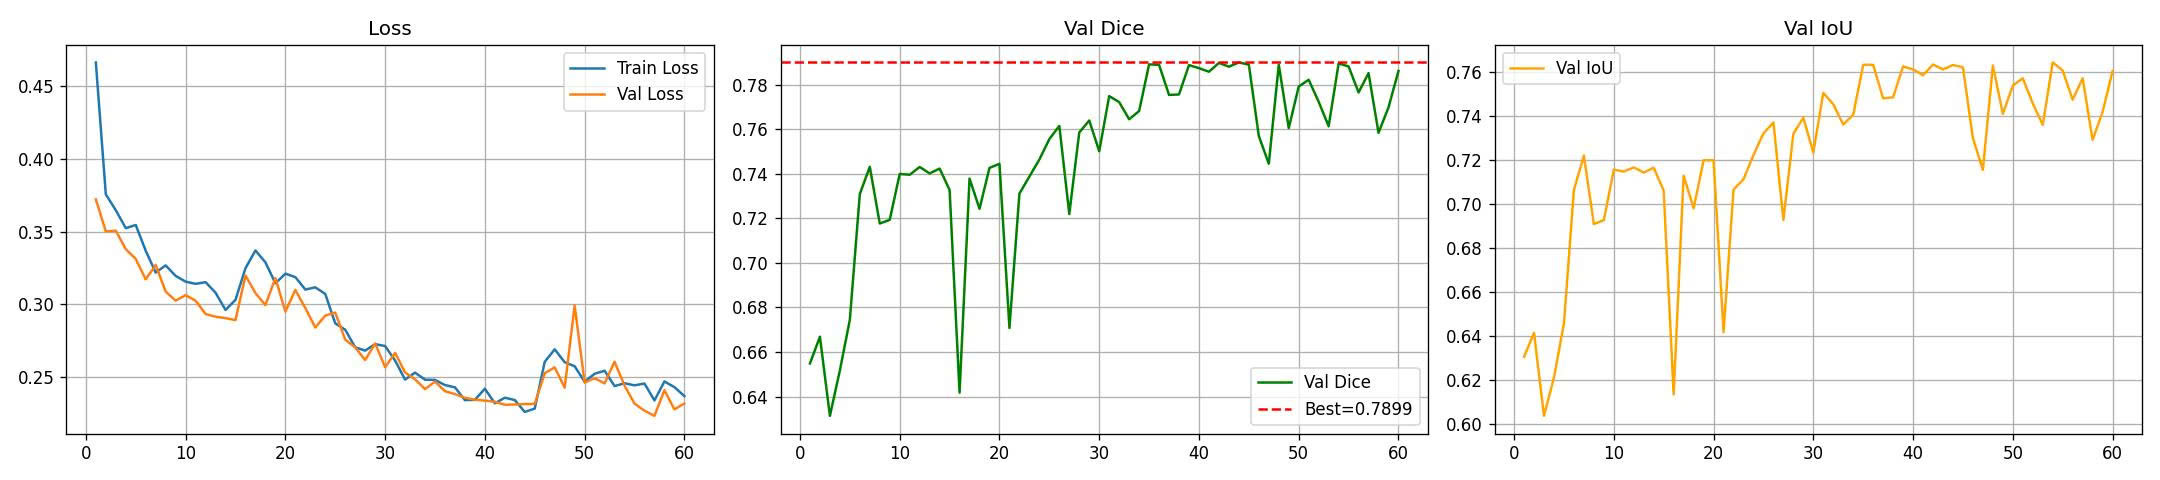
\includegraphics[width=\textwidth]{Figures/Gallery/m3_unetppeffb2_history.jpg}
    \caption{Lịch sử huấn luyện U-Net++ (EfficientNet-B2).}
    \label{fig:hist_unetpp_effb2}
\end{figure}

\begin{figure}[htbp]
    \centering
    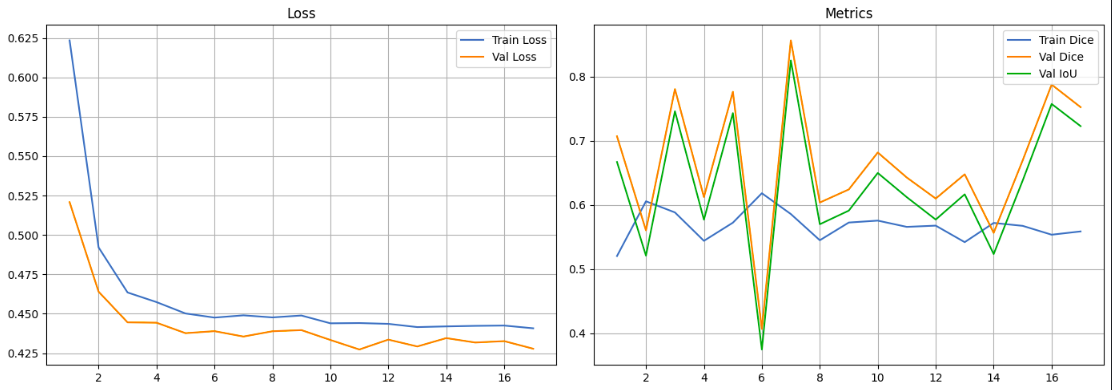
\includegraphics[width=\textwidth]{Figures/Chapter/Chapter6.png}
    \caption{Lịch sử huấn luyện ResUNet (ResNet-34).}
    \label{fig:hist_resunet}
\end{figure}

\FloatBarrier

\subsection{Kết quả dự đoán định tính}

\begin{figure}[H]
    \centering
    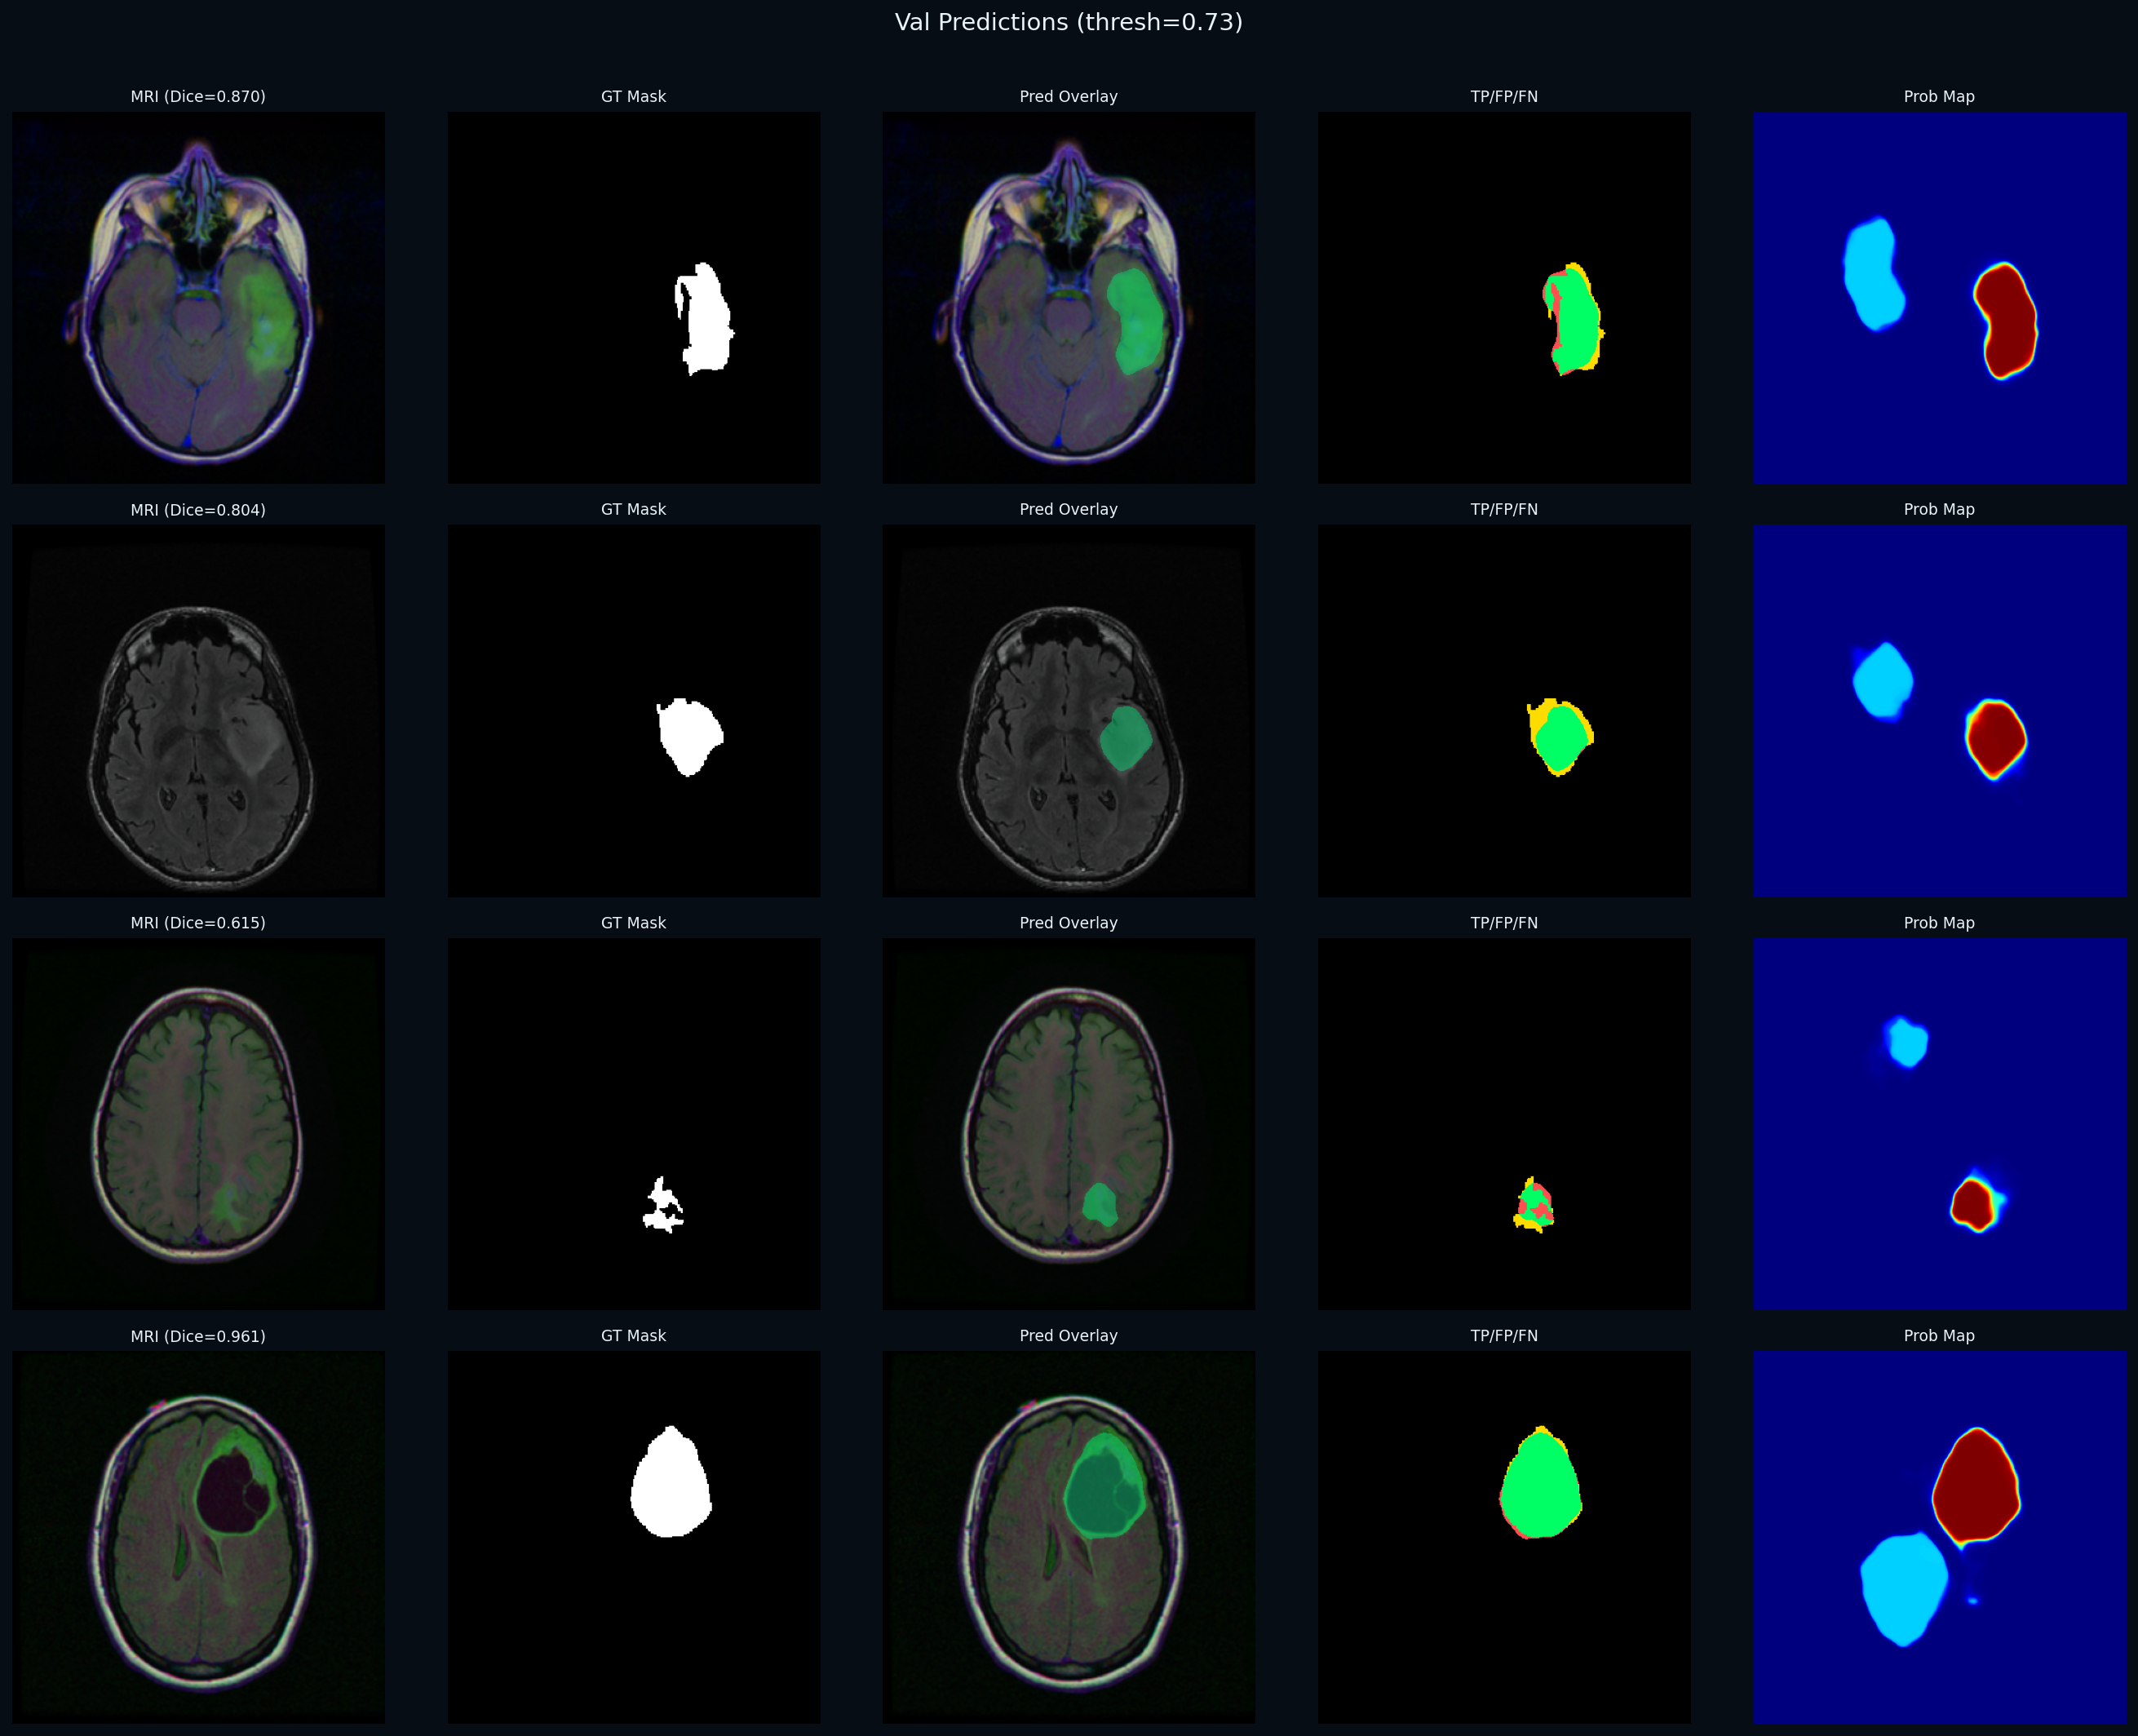
\includegraphics[width=0.85\textwidth,height=0.22\textheight,keepaspectratio]{Figures/Gallery/m1_uneteffb2_preds.png}
    \caption{Mẫu dự đoán của U-Net (EfficientNet-B2).}
\end{figure}

\begin{figure}[H]
    \centering
    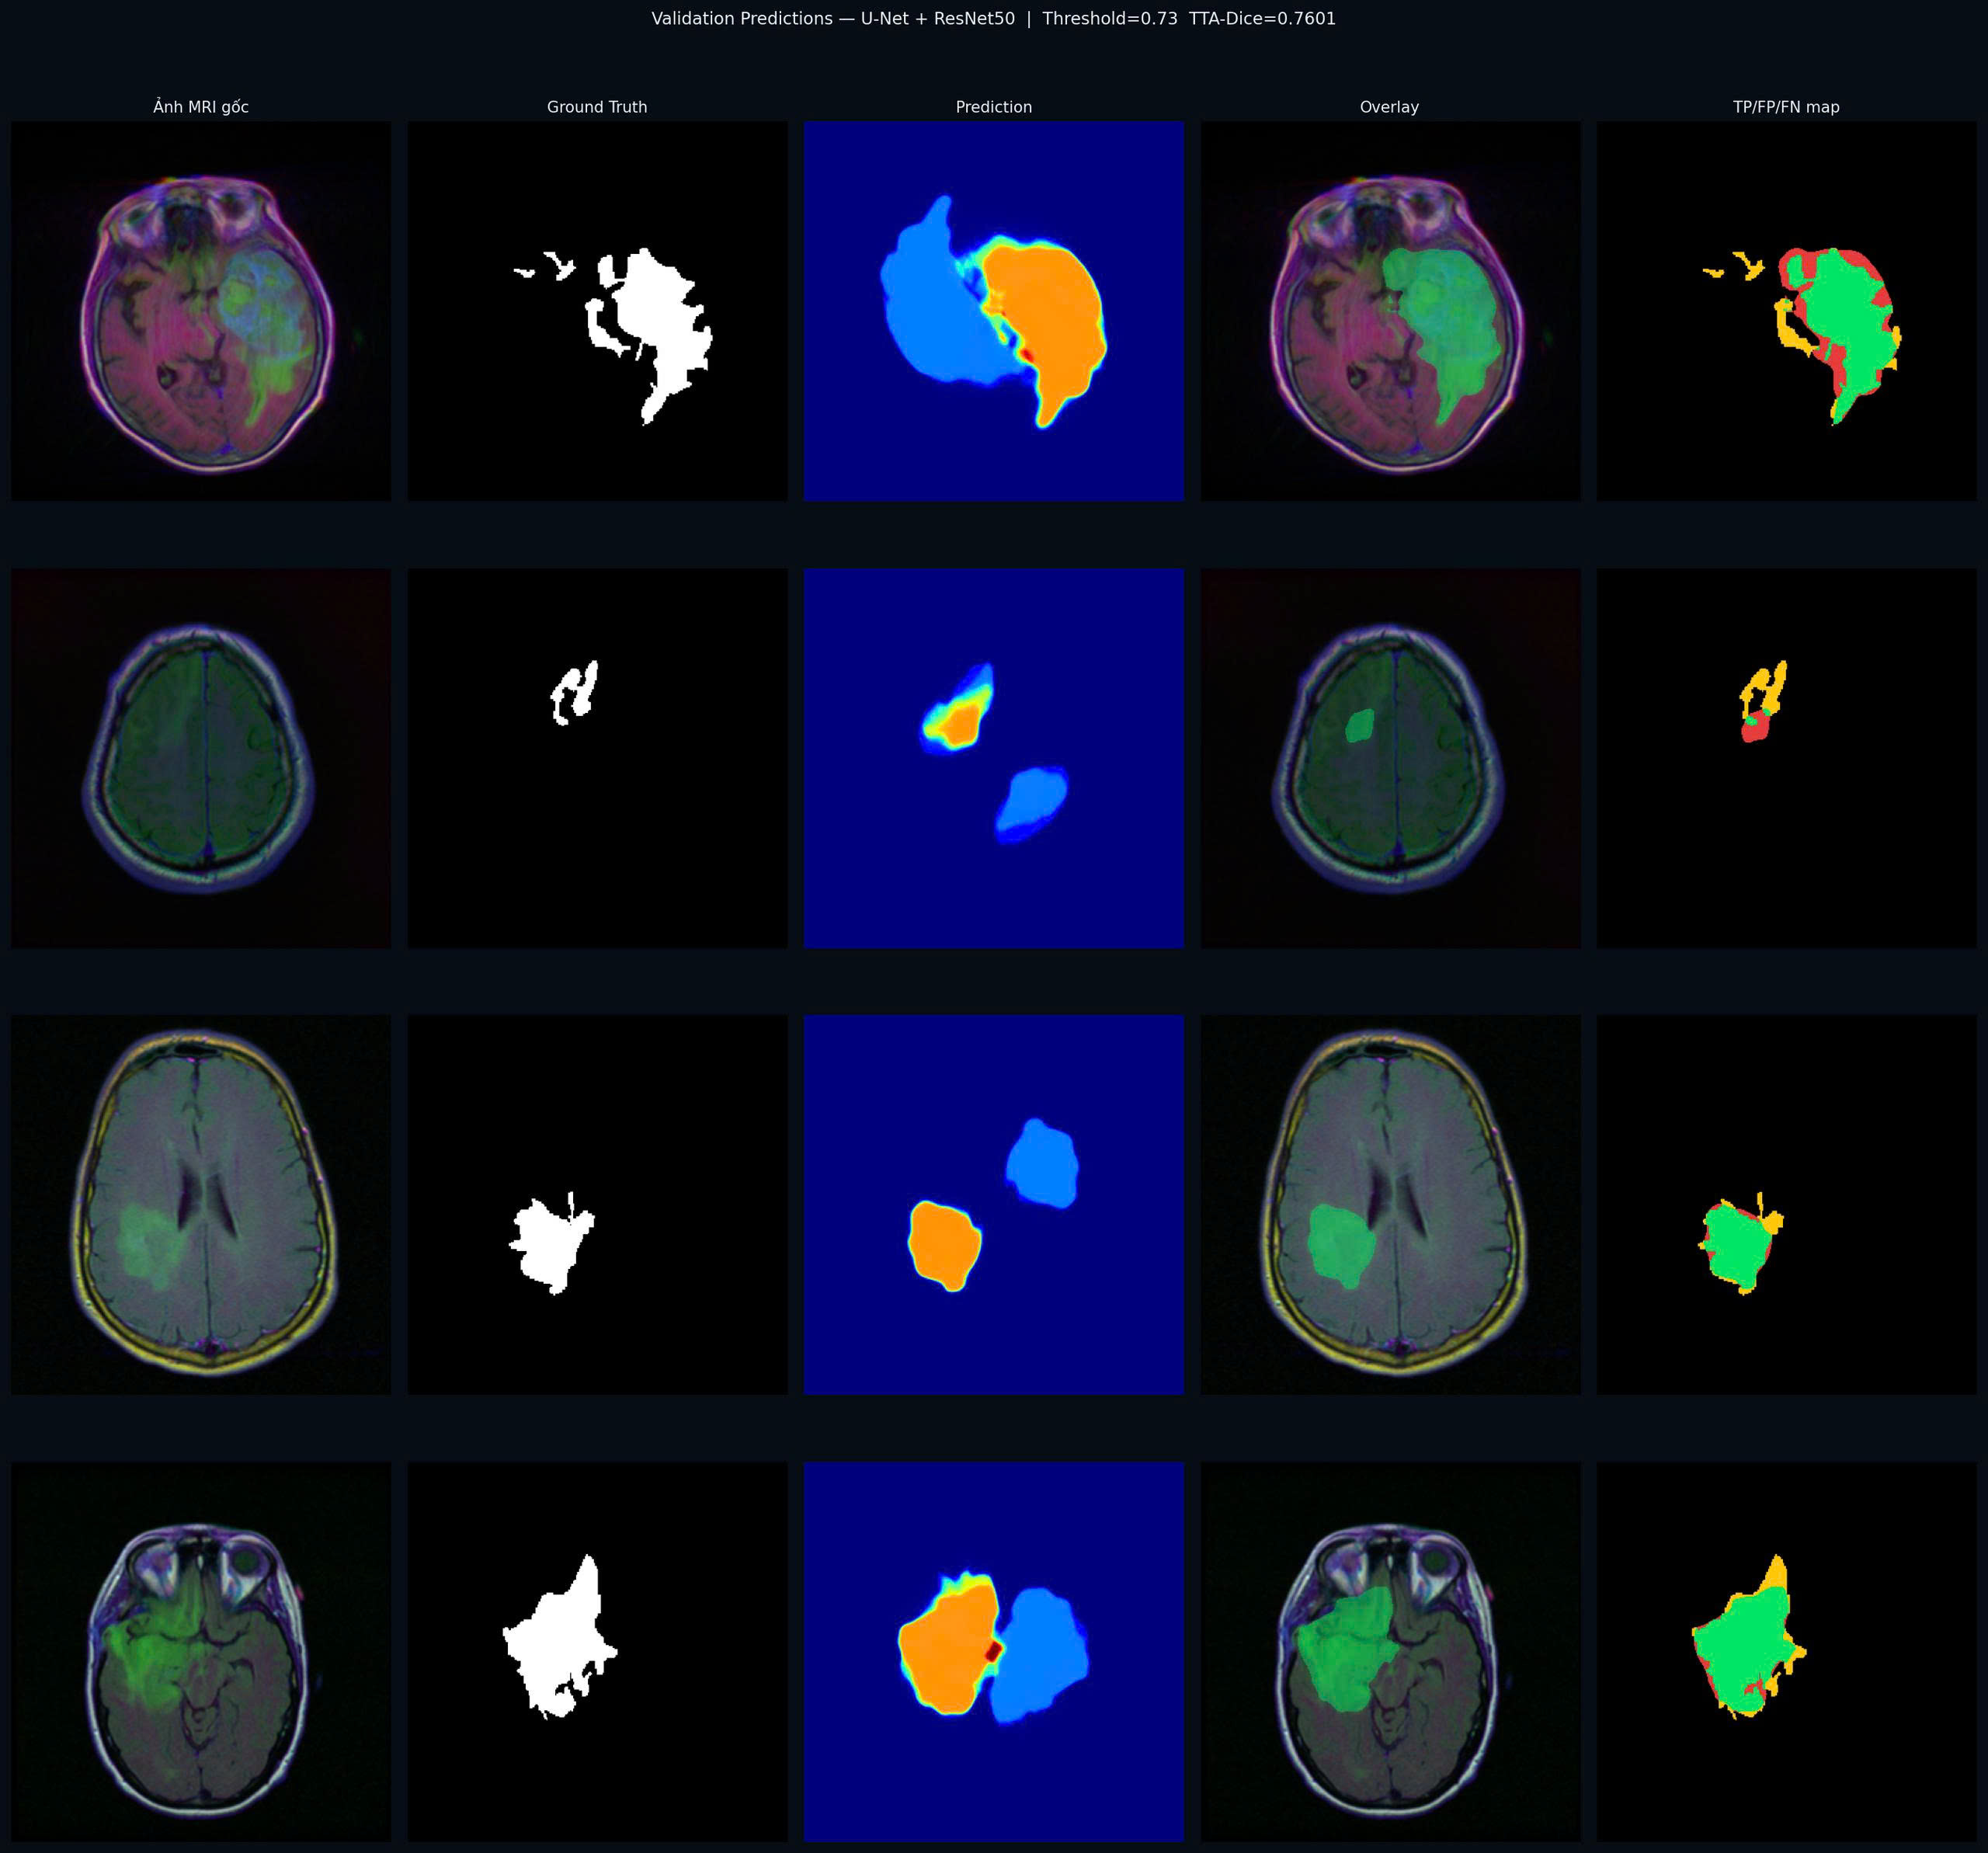
\includegraphics[width=0.85\textwidth,height=0.22\textheight,keepaspectratio]{Figures/Gallery/m2_unetresnet50_preds.jpg}
    \caption{Mẫu dự đoán của U-Net (ResNet-50).}
\end{figure}

\begin{figure}[H]
    \centering
    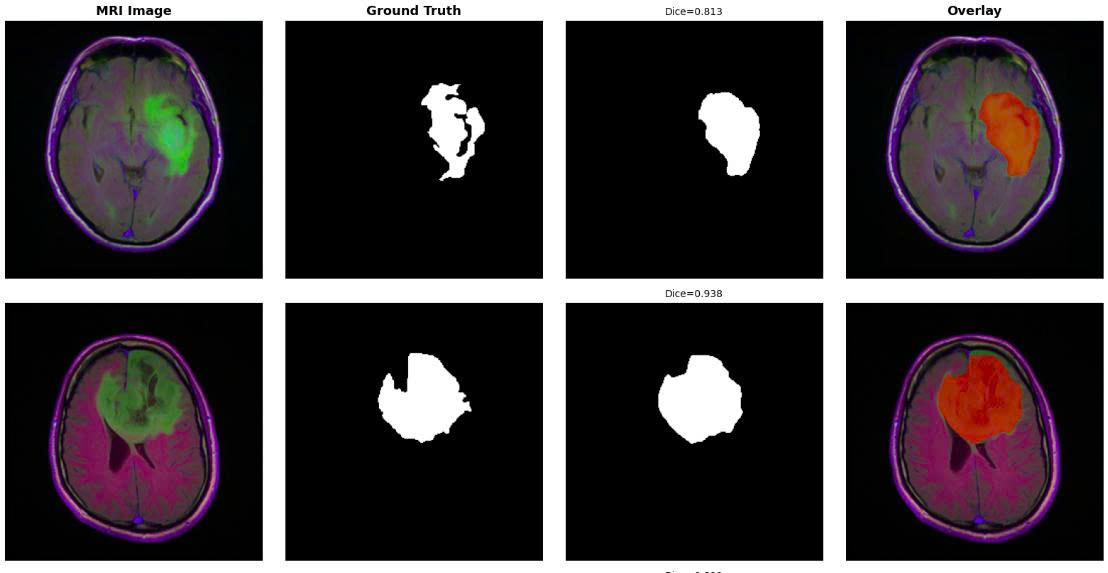
\includegraphics[width=0.85\textwidth,height=0.22\textheight,keepaspectratio]{Figures/Gallery/m3_unetppeffb2_preds.jpg}
    \caption{Mẫu dự đoán của U-Net++ (EfficientNet-B2).}
\end{figure}

\begin{figure}[H]
    \centering
    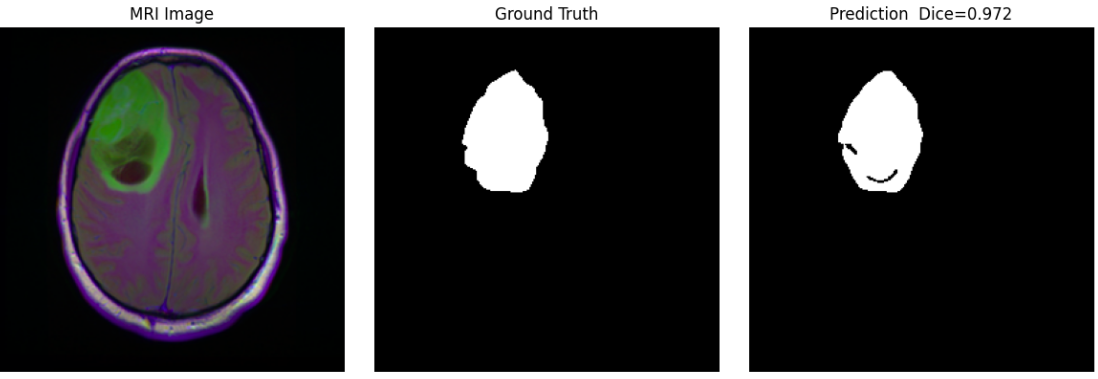
\includegraphics[width=0.85\textwidth,height=0.22\textheight,keepaspectratio]{Figures/Chapter/Chapter7.png}
    \caption{Mẫu dự đoán của ResUNet (ResNet-34).}
\end{figure}
\subsection{Phân tích và lựa chọn mô hình}

Dựa trên kết quả benchmark đầy đủ, \textbf{ResUNet + ResNet-34} được lựa chọn là mô hình triển khai chính trong hệ thống BrainSeg-XAI vì các lý do sau:

\begin{sloppypar}
\begin{enumerate}
    \item \textbf{DiCe cao nhất (0.8846):} Vượt tất cả các kiến trúc còn lại với biên độ lớn ($+$10.5 điểm tuyệt đối so với U-Net). Đây là số liệu trên tập test thực tế, không phải validation.
    \item \textbf{Recall vượt trội (0.8764):} Trong chẩn đoán u não, bỏ sót khối u (FN) là lỗi nghiêm trọng hơn báo dương giả (FP). Recall 0.8764 đảm bảo hệ thống phát hiện được phần lớn vùng bệnh lý.
    \item \textbf{IoU 0.7931 -- ngưỡng lâm sàng có ý nghĩa:} IoU $> 0.75$ thường được coi là mức phân đoạn tốt trong y tế. Ba mô hình còn lại đều dưới ngưỡng này.
    \item \textbf{Encoder nhẹ, inference nhanh:} ResNet-34 có ít tham số hơn EfficientNet-B2 và ResNet-50, phù hợp triển khai trên CPU không có GPU.
    \item \textbf{Ngưỡng auto-tuned 0.45:} Ngưỡng thấp hơn 0.5 giúp mô hình có xu hướng phát hiện nhiều vùng hơn, ưu tiên Recall -- chiến lược hợp lý về mặt lâm sàng.
\end{enumerate}
\end{sloppypar}

\section{Trực quan hóa Grad-CAM}

Bản đồ Grad-CAM trực quan hóa vùng ảnh ảnh hưởng đến quyết định phân đoạn. Phân tích định tính cho thấy:

\begin{itemize}
    \item Đối với ảnh có khối u rõ, bản đồ nhiệt tập trung chính xác vào vùng tăng tín hiệu tương ứng với khối u.
    \item Đối với ảnh không có khối u, Grad-CAM phân tán đều trên nhiều vùng, không có điểm nóng rõ ràng -- xác nhận mô hình không ``bịa đặt'' khối u giả.
    \item Một số trường hợp Grad-CAM kích hoạt vào cả vùng não khỏe mạnh lân cận khối u, phản ánh việc mô hình sử dụng ngữ cảnh không gian khi đưa ra quyết định.
\end{itemize}

Đây là hành vi mong đợi: Grad-CAM không chỉ hiển thị vùng khối u mà hiển thị vùng ảnh hưởng đến quyết định phân đoạn toàn cục.

\section{Phân tích bộ máy luật rủi ro}

Trên tập kiểm thử, phân bố điểm rủi ro phản ánh đặc điểm bộ dữ liệu LGG:
\begin{itemize}
    \item Phần lớn trường hợp rơi vào mức \textit{Thấp} hoặc \textit{Trung bình}, phù hợp với đặc tính u độ thấp (LGG) vốn phát triển chậm và ít xâm lấn hơn so với GBM.
    \item Các trường hợp được phân loại \textit{Cao} hoặc \textit{Rất cao} thường là khối u lớn, đa ổ hoặc có dịch chuyển đường giữa đáng kể.
    \item Quy tắc đóng góp điểm nhiều nhất trong dữ liệu LGG: R6 (diện tích tuyệt đối) và R2 (bất đối xứng hình dạng).
\end{itemize}

Điều quan trọng cần lưu ý là hệ thống luật không được xác thực lâm sàng chính thức và chỉ mang tính hỗ trợ tham khảo.

\section{Kiểm thử hệ thống end-to-end}

Hệ thống được kiểm thử bằng cách khởi động backend FastAPI và gọi API trực tiếp. Dưới đây là kết quả thực tế thu được từ endpoint \texttt{POST /api/v1/predict} ở chế độ demo (không có file weights huấn luyện):

\begin{table}[h!]
    \centering
    \caption{Kết quả kiểm thử hệ thống end-to-end trên CPU.}
    \label{tab:e2e_test}
    \begin{tabular}{l l l}
        \toprule
        \tabhead{Kịch bản} & \tabhead{Kết quả} & \tabhead{HTTP Status} \\
        \midrule
        File ảnh PNG hợp lệ          & JSON đầy đủ, pipeline chạy   & 200 OK \\
        File không phải ảnh          & Lỗi, thông báo rõ ràng       & 400 \\
        File $> 20$ MB               & Từ chối                      & 413 \\
        Không có file weights        & Demo mode, pipeline đầy đủ   & 200 OK \\
        \midrule
        \texttt{GET /api/v1/health}  & \texttt{\{"status":"ok"\}}   & 200 OK \\
        \bottomrule
    \end{tabular}
\end{table}

\subsection{Ví dụ response API thực tế}

Kết quả JSON trả về từ một request thực (demo mode, trọng số ngẫu nhiên) có cấu trúc như sau. Trường \texttt{features} chứa vector đặc trưng hình thái đầy đủ, và trường \texttt{risk} chứa đánh giá rủi ro có cấu trúc:

\begin{lstlisting}[style=plaintext, caption={Vi du response JSON tu POST /api/v1/predict (truong base64 da luoc bo)}]
{
  "features": {
    "tumor_detected":      true,
    "tumor_area_px":       20884,
    "tumor_area_cm2":      183.55,
    "occupancy_ratio":     31.87,
    "num_regions":         1073,
    "shape_irregularity":  0.9976,
    "compactness":         0.0024,
    "boundary_complexity": 72.0239,
    "midline_shift":       false,
    "location":            "thuy dinh/thai duong, trung tam",
    "centroid_x":          127.9,
    "centroid_y":          133.7
  },
  "risk": {
    "risk_level":  "Rat cao",
    "risk_score":  100,
    "severity":    "Nguy kich",
    "risk_color":  "#ff2d55",
    "fired_rules": [
      "Ty le chiem vung nao rat cao (31.87% > 20%)",
      "Hinh dang khoi u rat bat doi xung (irr=1.00)",
      "Duong bien khoi u rat phuc tap (complexity=72.0)",
      "Phat hien nhieu vung khoi u (1073 vung)",
      "Dien tich khoi u rat lon (183.55 cm2)"
    ],
    "recommendations": [
      "KHAN CAP: Can nhap vien va can thiep ngay lap tuc",
      "Can can thiep phau thuat khan cap",
      "Sinh thiet de xac dinh tinh ac tinh",
      "Chi dinh PET-CT de danh gia do xam lan"
    ],
    "explanation": "He thong phan tich 5 dac trung y khoa va
      kich hoat 5 co nguy co. Diem nguy co: 100/100.
      Phan loai: Nguy kich."
  }
}
\end{lstlisting}

Lưu ý: response trên là từ demo mode (trọng số ngẫu nhiên) nên các giá trị đặc trưng không phản ánh thực tế lâm sàng. Với model đã huấn luyện trên bộ dữ liệu LGG, kết quả phân đoạn sẽ khớp với vùng tín hiệu bất thường thực tế trên ảnh MRI.



%----------------------------------------------------------------------------------------
\section{Hạn chế hiện tại}
%----------------------------------------------------------------------------------------

\textbf{1. Phạm vi dữ liệu hạn hẹp.}
Hệ thống được huấn luyện và đánh giá trên bộ dữ liệu LGG thuần nhất. Hiệu suất trên dữ liệu GBM, u di căn hay các loại u khác chưa được kiểm chứng.

\textbf{2. Xử lý ảnh 2D đơn lẻ.}
Hệ thống chỉ xử lý từng lát cắt MRI riêng lẻ, không tận dụng thông tin không gian 3D từ toàn bộ sequence, giới hạn khả năng ước lượng thể tích khối u.

\textbf{3. Bộ máy luật chưa được xác thực lâm sàng.}
Các ngưỡng và trọng số điểm trong bộ máy luật được xác định theo tài liệu tham khảo, chưa trải qua xác thực prospective với bác sĩ chuyên khoa.

\textbf{4. Thiếu đánh giá calibration.}
Mô hình chưa được kiểm tra độ hiệu chỉnh xác suất: xác suất sigmoid đầu ra có thực sự phản ánh tần suất dự đoán đúng không?

\textbf{5. Phụ thuộc chất lượng ảnh đầu vào.}
Hệ thống chưa có cơ chế phát hiện ảnh chất lượng kém (nhiễu cao, thiếu tương phản) và chưa thực hiện chuẩn hóa cường độ theo từng thiết bị MRI.

%----------------------------------------------------------------------------------------
\section{Hướng phát triển}
%----------------------------------------------------------------------------------------

\subsection{Mở rộng sang phân đoạn 3D}

Bước phát triển tự nhiên là xử lý toàn bộ sequence MRI dưới dạng khối 3D. Các kiến trúc như 3D U-Net hoặc nnU-Net cho phép học đặc trưng không gian ba chiều, cải thiện độ chính xác phân đoạn và tính được thể tích khối u trực tiếp.

\subsection{Đa phương thức và đa chuỗi xung}

Kết hợp đồng thời nhiều chuỗi xung MRI (T1, T2, FLAIR, T1-Gd) như chuẩn của cuộc thi BraTS \cite{Menze2015} cho phép khai thác tương quan thông tin, cải thiện độ chính xác phân đoạn các tiểu vùng (tumor core, enhancing tumor, edema).

\subsection{Xác thực lâm sàng}

Để hướng tới ứng dụng thực tế:
\begin{itemize}
    \item Xác thực prospective các ngưỡng trong bộ máy luật với bác sĩ chuyên khoa thần kinh.
    \item Đánh giá inter-rater agreement giữa chú thích của hệ thống và bác sĩ.
    \item Tuân thủ quy định y tế như FDA 510(k) hoặc CE Mark tùy thị trường mục tiêu.
\end{itemize}

\subsection{Tích hợp PACS và giao diện mở rộng}

Tích hợp với hệ thống PACS (Picture Archiving and Communication System) giúp nhận ảnh DICOM trực tiếp từ thiết bị MRI. Giao diện có thể mở rộng hỗ trợ MPR viewer (xem lát cắt 3D), xuất báo cáo PDF và lưu trữ kết quả theo bệnh nhân.

\subsection{Cải thiện khả năng giải thích}

Ngoài Grad-CAM, có thể tích hợp thêm SHAP để giải thích đóng góp từng đặc trưng hình thái vào điểm rủi ro; attention maps từ kiến trúc transformer; và uncertainty quantification (Monte Carlo Dropout) để ước tính độ không chắc chắn của dự đoán.

%----------------------------------------------------------------------------------------
\section{Kết luận chung}
%----------------------------------------------------------------------------------------

BrainSeg-XAI thể hiện rằng việc xây dựng một hệ thống AI y tế \textit{có thể giải thích được} là khả thi với các công nghệ nguồn mở hiện có. Hệ thống không chỉ tạo ra mặt nạ phân đoạn mà còn cung cấp cơ chế giải thích đa lớp: Grad-CAM ở cấp độ pixel, đặc trưng hình thái ở cấp độ vùng, và đánh giá rủi ro có cấu trúc ở cấp độ lâm sàng. Đây là hướng tiếp cận phù hợp với xu hướng phát triển của AI y tế: không thay thế bác sĩ mà trang bị cho họ công cụ phân tích mạnh mẽ và minh bạch hơn để đưa ra quyết định lâm sàng chính xác.



%----------------------------------------------------------------------------------------
%	PHẦN 13: TÀI LIỆU THAM KHẢO
%----------------------------------------------------------------------------------------

\begin{spacing}{1.15}
	\printbibliography[heading=bibintoc, title=Tài liệu tham khảo]
\end{spacing}


%----------------------------------------------------------------------------------------
%	PHẦN 14: PHỤ LỤC
%----------------------------------------------------------------------------------------

\appendix

% Phụ lục A: Mã nguồn hệ thống BrainSeg-XAI

\chapter{Mã nguồn hệ thống BrainSeg-XAI}

\label{AppendixA}

%----------------------------------------------------------------------------------------

Phụ lục này trình bày toàn bộ mã nguồn của các module cốt lõi trong hệ thống BrainSeg-XAI.
Mã nguồn được tổ chức theo cấu trúc thư mục thực tế của dự án.

%----------------------------------------------------------------------------------------
\section{Backend -- Ứng dụng FastAPI chính (\texttt{app/main.py})}
%----------------------------------------------------------------------------------------

\begin{lstlisting}[style=codePython, caption={FastAPI -- Khoi tao app va CORS middleware (app/main.py)}]
from fastapi import FastAPI
from fastapi.middleware.cors import CORSMiddleware
from app.api.predict import router as predict_router

app = FastAPI(
    title="Brain Tumor AI API",
    description="He thong AI phan tich va danh gia khoi u nao tu anh MRI",
    version="1.0.0",
)

app.add_middleware(
    CORSMiddleware,
    allow_origins=["*"],
    allow_credentials=True,
    allow_methods=["*"],
    allow_headers=["*"],
)

app.include_router(predict_router, prefix="/api/v1")

@app.get("/")
async def root():
    return {
        "name": "Brain Tumor AI",
        "version": "1.0.0",
        "docs": "/docs",
    }
\end{lstlisting}

%----------------------------------------------------------------------------------------
\section{Backend -- Endpoint dự đoán (\texttt{app/api/predict.py})}
%----------------------------------------------------------------------------------------

\begin{lstlisting}[style=codePython, caption={REST API endpoint nhan anh MRI va tra ket qua phan tich (app/api/predict.py)}]
from fastapi import APIRouter, UploadFile, File, HTTPException
from app.services.inference import predict
from app.utils.image_utils import load_image_from_bytes

router = APIRouter()

@router.post("/predict")
async def predict_endpoint(file: UploadFile = File(...)):
    if not file.content_type.startswith("image/"):
        raise HTTPException(
            status_code=400,
            detail="Chi chap nhan file anh.")

    raw = await file.read()
    if len(raw) > 20 * 1024 * 1024:
        raise HTTPException(
            status_code=413,
            detail="File anh qua lon (toi da 20MB).")

    try:
        img_rgb = load_image_from_bytes(raw)
    except ValueError as e:
        raise HTTPException(status_code=422, detail=str(e))

    try:
        result = predict(img_rgb)
    except Exception as e:
        raise HTTPException(
            status_code=500,
            detail=f"Loi xu ly mo hinh: {str(e)}")

    return result

@router.get("/health")
async def health():
    return {"status": "ok",
            "message": "Brain Tumor AI API dang hoat dong"}
\end{lstlisting}

%----------------------------------------------------------------------------------------
\section{Backend -- Tiện ích xử lý ảnh (\texttt{app/utils/image\_utils.py})}
%----------------------------------------------------------------------------------------

\begin{lstlisting}[style=codePython, caption={Tien xu ly anh MRI: doc, resize 256x256, chuan hoa ImageNet (app/utils/image\_utils.py)}]
import cv2
import numpy as np
from PIL import Image
import io
import base64

TARGET_SIZE = (256, 256)
MEAN = [0.485, 0.456, 0.406]   # ImageNet mean
STD  = [0.229, 0.224, 0.225]   # ImageNet std

def load_image_from_bytes(raw: bytes) -> np.ndarray:
    arr = np.frombuffer(raw, dtype=np.uint8)
    img = cv2.imdecode(arr, cv2.IMREAD_COLOR)
    if img is None:
        raise ValueError(
            "Khong the doc anh. Vui long thu lai voi file anh hop le.")
    return cv2.cvtColor(img, cv2.COLOR_BGR2RGB)

def preprocess(img_rgb: np.ndarray):
    """Tra ve (tensor NCHW float32, original_rgb resized 256x256)"""
    import torch
    resized = cv2.resize(img_rgb, TARGET_SIZE,
                         interpolation=cv2.INTER_LINEAR)
    norm = resized.astype(np.float32) / 255.0
    for c in range(3):
        norm[:, :, c] = (norm[:, :, c] - MEAN[c]) / STD[c]
    tensor = torch.from_numpy(
        norm.transpose(2, 0, 1)).unsqueeze(0)  # 1x3xHxW
    return tensor, resized

def mask_to_binary(logits_tensor) -> np.ndarray:
    import torch
    prob = torch.sigmoid(logits_tensor).squeeze().cpu().numpy()
    return (prob > 0.5).astype(np.uint8)

def ndarray_to_b64(arr: np.ndarray, ext: str = "png") -> str:
    pil = Image.fromarray(arr.astype(np.uint8))
    buf = io.BytesIO()
    pil.save(buf, format=ext.upper())
    return base64.b64encode(buf.getvalue()).decode()

def apply_colormap_heatmap(gray: np.ndarray) -> np.ndarray:
    """gray: HxW float [0,1] -> RGB uint8 (JET colormap)"""
    gray_u8 = (gray * 255).clip(0, 255).astype(np.uint8)
    colored = cv2.applyColorMap(gray_u8, cv2.COLORMAP_JET)
    return cv2.cvtColor(colored, cv2.COLOR_BGR2RGB)

def overlay_mask(img_rgb: np.ndarray, mask: np.ndarray,
                 alpha: float = 0.45) -> np.ndarray:
    overlay = img_rgb.copy()
    overlay[mask == 1] = [255, 80, 80]
    return cv2.addWeighted(img_rgb, 1 - alpha, overlay, alpha, 0)

def overlay_heatmap(img_rgb: np.ndarray, heatmap_rgb: np.ndarray,
                    alpha: float = 0.5) -> np.ndarray:
    return cv2.addWeighted(img_rgb, 1 - alpha, heatmap_rgb, alpha, 0)
\end{lstlisting}

%----------------------------------------------------------------------------------------
\section{Backend -- Định nghĩa mô hình (\texttt{app/models/unet.py})}
%----------------------------------------------------------------------------------------

\begin{lstlisting}[style=codePython, caption={Vanilla UNet va SMP wrapper -- ho tro U-Net va U-Net++ (app/models/unet.py)}]
import torch
import torch.nn as nn
import torch.nn.functional as F

# --- 1. Vanilla U-Net (backward-compat voi weight cu) ---------------
class DoubleConv(nn.Module):
    def __init__(self, in_ch, out_ch):
        super().__init__()
        self.conv = nn.Sequential(
            nn.Conv2d(in_ch, out_ch, 3, padding=1, bias=False),
            nn.BatchNorm2d(out_ch), nn.ReLU(inplace=True),
            nn.Conv2d(out_ch, out_ch, 3, padding=1, bias=False),
            nn.BatchNorm2d(out_ch), nn.ReLU(inplace=True),
        )
    def forward(self, x): return self.conv(x)

class Down(nn.Module):
    def __init__(self, ic, oc):
        super().__init__()
        self.pool_conv = nn.Sequential(
            nn.MaxPool2d(2), DoubleConv(ic, oc))
    def forward(self, x): return self.pool_conv(x)

class Up(nn.Module):
    def __init__(self, ic, oc):
        super().__init__()
        self.up   = nn.ConvTranspose2d(ic, ic // 2, 2, stride=2)
        self.conv = DoubleConv(ic, oc)
    def forward(self, x1, x2):
        x1 = self.up(x1)
        dy = x2.size(2) - x1.size(2)
        dx = x2.size(3) - x1.size(3)
        x1 = F.pad(x1, [dx//2, dx-dx//2, dy//2, dy-dy//2])
        return self.conv(torch.cat([x2, x1], 1))

class UNet(nn.Module):
    def __init__(self, n_channels=3, n_classes=1,
                 features=[64, 128, 256, 512]):
        super().__init__()
        f = features
        self.inc   = DoubleConv(n_channels, f[0])
        self.down1 = Down(f[0], f[1])
        self.down2 = Down(f[1], f[2])
        self.down3 = Down(f[2], f[3])
        self.down4 = Down(f[3], f[3]*2)
        self.up1   = Up(f[3]*2, f[3])
        self.up2   = Up(f[3],   f[2])
        self.up3   = Up(f[2],   f[1])
        self.up4   = Up(f[1],   f[0])
        self.outc  = nn.Conv2d(f[0], n_classes, 1)

    def forward(self, x):
        x1 = self.inc(x)
        x2 = self.down1(x1)
        x3 = self.down2(x2)
        x4 = self.down3(x3)
        x5 = self.down4(x4)
        x  = self.up1(x5, x4)
        x  = self.up2(x,  x3)
        x  = self.up3(x,  x2)
        x  = self.up4(x,  x1)
        return self.outc(x)

# --- 2. SMP wrapper --------------------------------------------------
def build_smp_model(arch="unetplusplus",
                    encoder="efficientnet-b4",
                    encoder_weights="imagenet",
                    n_classes=1):
    """
    arch    : 'unetplusplus' | 'unet' | 'deeplabv3plus' | 'fpn' | 'manet'
    encoder : 'efficientnet-b4' | 'resnet50' | 'resnet34' | ...
    """
    try:
        import segmentation_models_pytorch as smp
    except ImportError:
        raise ImportError(
            "segmentation-models-pytorch chua duoc cai.\n"
            "Chay: pip install segmentation-models-pytorch timm")
    return smp.create_model(
        arch,
        encoder_name=encoder,
        encoder_weights=encoder_weights,
        in_channels=3,
        classes=n_classes,
        activation=None,
    )

# --- 3. Auto-loader --------------------------------------------------
def get_model(arch="unetplusplus", encoder="efficientnet-b4",
              n_classes=1, pretrained=True):
    try:
        model = build_smp_model(
            arch=arch, encoder=encoder,
            encoder_weights="imagenet" if pretrained else None,
            n_classes=n_classes)
        print(f"[Model] Dung SMP -- arch={arch}, encoder={encoder}")
        return model, "smp"
    except Exception as e:
        print(f"[Model] SMP khong kha dung ({e}), fallback UNet.")
        return UNet(n_channels=3, n_classes=n_classes), "vanilla"
\end{lstlisting}

%----------------------------------------------------------------------------------------
\section{Backend -- Dịch vụ suy luận (\texttt{app/services/inference.py})}
%----------------------------------------------------------------------------------------

\begin{lstlisting}[style=codePython, caption={Lazy model loading, auto-detect checkpoint va dieu phoi prediction pipeline (app/services/inference.py)}]
import torch
import numpy as np
from pathlib import Path

from app.models.unet import get_model, UNet
from app.utils.image_utils import (
    preprocess, mask_to_binary,
    apply_colormap_heatmap, overlay_mask, overlay_heatmap,
    ndarray_to_b64,
)
from app.xai.gradcam import GradCAM, get_target_layer
from app.services.feature_extraction import extract_features
from app.rules.medical_rules import evaluate_risk

WEIGHTS_PATH = (Path(__file__).parent.parent.parent
                / "weights" / "unet_best.pth")
DEVICE = torch.device("cuda" if torch.cuda.is_available() else "cpu")

_model      = None
_model_type = "vanilla"
_gradcam    = None

def convert_numpy(obj):
    if isinstance(obj, (np.bool_, bool)):    return bool(obj)
    if isinstance(obj, np.integer):          return int(obj)
    if isinstance(obj, np.floating):         return float(obj)
    if isinstance(obj, np.ndarray):          return obj.tolist()
    if isinstance(obj, dict):
        return {k: convert_numpy(v) for k, v in obj.items()}
    if isinstance(obj, (list, tuple)):
        return [convert_numpy(v) for v in obj]
    return obj

def _load_model():
    global _model, _model_type, _gradcam
    if _model is not None:
        return

    if not WEIGHTS_PATH.exists():
        print("[WARN] Weights not found -- demo mode (random weights).")
        model, mtype = get_model(pretrained=False)
        model.to(DEVICE).eval()
        _model      = model
        _model_type = mtype
        _gradcam    = GradCAM(model, get_target_layer(model, mtype))
        return

    ckpt = torch.load(WEIGHTS_PATH, map_location=DEVICE)

    arch    = (ckpt.get("arch",    "unetplusplus")
               if isinstance(ckpt, dict) else "unetplusplus")
    encoder = (ckpt.get("encoder", "efficientnet-b4")
               if isinstance(ckpt, dict) else "efficientnet-b4")

    if isinstance(ckpt, dict) and "model_state_dict" in ckpt:
        sd = ckpt["model_state_dict"]
    elif isinstance(ckpt, dict) and "state_dict" in ckpt:
        sd = ckpt["state_dict"]
    elif isinstance(ckpt, dict) and any(
        k.startswith("encoder") or k.startswith("decoder")
        for k in ckpt.keys()
    ):
        sd = ckpt
        arch, encoder = "unetplusplus", "efficientnet-b4"
    else:
        sd = ckpt

    keys = list(sd.keys()) if isinstance(sd, dict) else []
    is_vanilla = any(
        k.startswith("inc.") or k.startswith("down")
        or k.startswith("up")
        for k in keys)

    if is_vanilla:
        model, mtype = UNet(n_channels=3, n_classes=1), "vanilla"
        print(f"[Model] Load vanilla UNet tu {WEIGHTS_PATH}")
    else:
        try:
            model, mtype = get_model(
                arch=arch, encoder=encoder, pretrained=False)
            print(f"[Model] Load SMP {arch}/{encoder}")
        except Exception as e:
            print(f"[Model] SMP fail ({e}), thu vanilla UNet.")
            model, mtype = UNet(n_channels=3, n_classes=1), "vanilla"

    model.load_state_dict(sd, strict=False)
    model.to(DEVICE).eval()
    _model      = model
    _model_type = mtype
    _gradcam    = GradCAM(model, get_target_layer(model, mtype))
    print(f"[Model] Ready -- type={mtype}, device={DEVICE}")

def predict(img_rgb: np.ndarray) -> dict:
    _load_model()
    tensor, resized = preprocess(img_rgb)
    tensor = tensor.to(DEVICE)

    with torch.no_grad():
        logits = _model(tensor)

    mask = mask_to_binary(logits)

    try:
        cam = _gradcam.generate(tensor.clone())
    except Exception as e:
        print(f"[GradCAM] Error: {e}")
        cam = np.zeros(resized.shape[:2], dtype=np.float32)

    heatmap_rgb  = apply_colormap_heatmap(cam)
    mask_overlay = overlay_mask(resized, mask)
    cam_overlay  = overlay_heatmap(resized, heatmap_rgb)

    mask_vis = np.zeros((*mask.shape, 3), dtype=np.uint8)
    mask_vis[mask == 1] = [0, 255, 136]

    features = extract_features(mask, mask.shape)
    risk     = evaluate_risk(features)

    return convert_numpy({
        "original_b64":    ndarray_to_b64(resized),
        "mask_b64":        ndarray_to_b64(mask_vis),
        "overlay_b64":     ndarray_to_b64(mask_overlay),
        "heatmap_b64":     ndarray_to_b64(heatmap_rgb),
        "cam_overlay_b64": ndarray_to_b64(cam_overlay),
        "features": features,
        "risk": {
            "risk_level":      risk.risk_level,
            "risk_score":      risk.risk_score,
            "severity":        risk.severity,
            "risk_color":      risk.risk_color,
            "fired_rules":     risk.fired_rules,
            "recommendations": risk.recommendations,
            "explanation":     risk.explanation,
        },
    })
\end{lstlisting}

%----------------------------------------------------------------------------------------
\section{Backend -- Module Grad-CAM (\texttt{app/xai/gradcam.py})}
%----------------------------------------------------------------------------------------

\begin{lstlisting}[style=codePython, caption={Trien khai Grad-CAM voi PyTorch forward/backward hooks (app/xai/gradcam.py)}]
import numpy as np
import torch
import torch.nn.functional as F

class GradCAM:
    def __init__(self, model: torch.nn.Module,
                 target_layer: torch.nn.Module):
        self.model        = model
        self.target_layer = target_layer
        self._features    = None
        self._grads       = None
        self._hooks       = []
        self._register()

    def _register(self):
        self._hooks.append(
            self.target_layer.register_forward_hook(
                self._save_features))
        self._hooks.append(
            self.target_layer.register_full_backward_hook(
                self._save_grads))

    def _save_features(self, m, inp, out):
        self._features = out.detach()

    def _save_grads(self, m, gi, go):
        self._grads = go[0].detach()

    def remove_hooks(self):
        for h in self._hooks:
            h.remove()

    def generate(self, input_tensor: torch.Tensor) -> np.ndarray:
        self.model.eval()
        input_tensor = input_tensor.detach().requires_grad_(True)

        output = self.model(input_tensor)
        score  = torch.sigmoid(output).sum()   # tong sigmoid cho phan doan nhi phan
        self.model.zero_grad()
        score.backward()

        if self._grads is None or self._features is None:
            return np.zeros(input_tensor.shape[-2:], dtype=np.float32)

        # Global Average Pooling tren gradient
        weights = self._grads.mean(dim=(2, 3), keepdim=True)
        cam = F.relu(
            (weights * self._features).sum(dim=1, keepdim=True))

        cam = F.interpolate(
            cam,
            size=input_tensor.shape[-2:],
            mode="bilinear",
            align_corners=False)
        cam = cam.squeeze().cpu().numpy()

        lo, hi = cam.min(), cam.max()
        if hi - lo > 1e-8:
            cam = (cam - lo) / (hi - lo)  # chuan hoa min-max
        else:
            cam = np.zeros_like(cam)
        return cam.astype(np.float32)

def get_target_layer(model, model_type: str = "vanilla"):
    """Chon layer de dang ky hook Grad-CAM theo loai model."""
    if model_type == "smp":
        try:
            return model.segmentation_head[0]
        except Exception:
            pass
        try:
            blocks = list(model.decoder.blocks)
            return blocks[-1].conv2[0]
        except Exception:
            pass
        convs = [m for m in model.modules()
                 if isinstance(m, torch.nn.Conv2d)]
        return convs[-2] if len(convs) >= 2 else convs[-1]
    else:
        # Vanilla UNet: layer truoc lop dau ra cuoi cung
        return model.up4.conv.conv[-3]
\end{lstlisting}

%----------------------------------------------------------------------------------------
\section[Backend -- Trích xuất đặc trưng]{Backend -- Trích xuất đặc trưng (\texttt{feature\_extraction.py})}
%----------------------------------------------------------------------------------------

\begin{lstlisting}[style=codePython, caption={Tinh toan dac trung hinh thai hoc tu mat na nhi phan (app/services/feature\_extraction.py)}]
import numpy as np
from scipy import ndimage
from skimage import measure

def extract_features(mask: np.ndarray, img_shape: tuple) -> dict:
    """
    mask      : binary HxW uint8
    img_shape : (H, W)
    Returns   : dict cac dac trung y khoa
    """
    H, W = img_shape
    total_pixels = H * W

    labeled, num_tumors = ndimage.label(mask)
    tumor_pixels    = int(mask.sum())
    occupancy_ratio = round(tumor_pixels / total_pixels * 100, 2)

    if tumor_pixels == 0:
        return {
            "tumor_detected":    False,
            "tumor_area_px":     0,
            "tumor_area_cm2":    0.0,
            "occupancy_ratio":   0.0,
            "num_regions":       0,
            "shape_irregularity": 0.0,
            "compactness":       0.0,
            "boundary_complexity": 0.0,
            "midline_shift":     False,
            "location":          "Khong phat hien khoi u",
            "centroid_x":        None,
            "centroid_y":        None,
        }

    # Chuyen doi px -> cm2 (MRI slice ~ 24cm x 24cm tai 256x256)
    px_to_cm = (24.0 / H) ** 2
    tumor_area_cm2 = round(tumor_pixels * px_to_cm, 2)

    # Dac trung hinh dang qua regionprops cua vung lon nhat
    props_list = measure.regionprops(labeled)
    props = max(props_list, key=lambda p: p.area)

    perimeter = props.perimeter if props.perimeter > 0 else 1
    area_p    = props.area
    compactness = round((4 * np.pi * area_p) / (perimeter ** 2), 4)
    shape_irregularity  = round(1.0 - compactness, 4)
    boundary_complexity = round(
        perimeter / (np.sqrt(area_p) + 1e-6), 4)

    cy, cx    = props.centroid
    cx_norm   = cx / W
    cy_norm   = cy / H

    h_loc = ("ben trai" if cx_norm < 0.45
             else "ben phai" if cx_norm > 0.55
             else "trung tam")
    v_loc = ("thuy tran" if cy_norm < 0.33
             else "thuy dinh/thai duong" if cy_norm < 0.66
             else "thuy cham/tieu nao")
    location = f"{v_loc}, {h_loc}"

    midline_shift = abs(cx_norm - 0.5) > 0.10

    return {
        "tumor_detected":    True,
        "tumor_area_px":     tumor_pixels,
        "tumor_area_cm2":    tumor_area_cm2,
        "occupancy_ratio":   occupancy_ratio,
        "num_regions":       num_tumors,
        "shape_irregularity": shape_irregularity,
        "compactness":       compactness,
        "boundary_complexity": boundary_complexity,
        "midline_shift":     midline_shift,
        "location":          location,
        "centroid_x":        round(float(cx), 1),
        "centroid_y":        round(float(cy), 1),
    }
\end{lstlisting}

%----------------------------------------------------------------------------------------
\section{Backend -- Bộ máy luật y khoa (\texttt{app/rules/medical\_rules.py})}
%----------------------------------------------------------------------------------------

\begin{lstlisting}[style=codePython, caption={Rule-based risk engine -- 6 quy tac, additive scoring, 4 muc rui ro (app/rules/medical\_rules.py)}]
from dataclasses import dataclass, field
from typing import List

@dataclass
class RuleResult:
    risk_level:      str   # "Thap" | "Trung binh" | "Cao" | "Rat cao"
    risk_score:      int   # 0-100
    severity:        str   # "Binh thuong" | "Nhe" | ... | "Nguy kich"
    risk_color:      str   # hex color cho UI
    fired_rules:     List[str] = field(default_factory=list)
    recommendations: List[str] = field(default_factory=list)
    explanation:     str = ""

def evaluate_risk(features: dict) -> RuleResult:
    if not features.get("tumor_detected", False):
        return RuleResult(
            risk_level="Thap", risk_score=0,
            severity="Binh thuong", risk_color="#00ff88",
            fired_rules=["Khong phat hien khoi u trong anh MRI"],
            recommendations=["Tiep tuc theo doi dinh ky",
                             "Chup MRI kiem tra sau 12 thang"],
            explanation="Khong phat hien bat ky vung bat thuong nao.")

    score = 0
    fired, recs = [], []

    occ   = features["occupancy_ratio"]
    irr   = features["shape_irregularity"]
    bnd   = features["boundary_complexity"]
    mid   = features["midline_shift"]
    n_reg = features["num_regions"]
    area  = features["tumor_area_cm2"]

    # Rule 1: Occupancy ratio
    if occ > 20:
        score += 30
        fired.append(f"Ty le chiem vung nao rat cao ({occ}% > 20%)")
        recs.append("Can can thiep phau thuat khan cap")
    elif occ > 10:
        score += 20
        fired.append(f"Ty le chiem vung nao cao ({occ}% > 10%)")
        recs.append("Hoi chan chuyen khoa than kinh ngay")
    elif occ > 5:
        score += 10
        fired.append(f"Ty le chiem vung nao o muc trung binh ({occ}%)")
        recs.append("Theo doi sat va chup MRI dinh ky 3 thang/lan")
    else:
        fired.append(f"Ty le chiem vung nao thap ({occ}%)")

    # Rule 2: Shape irregularity
    if irr > 0.7:
        score += 25
        fired.append(
            f"Hinh dang khoi u rat bat doi xung (irr={irr:.2f})")
        recs.append("Sinh thiet de xac dinh tinh ac tinh")
    elif irr > 0.5:
        score += 15
        fired.append(
            f"Hinh dang khoi u bat doi xung vua (irr={irr:.2f})")
    else:
        fired.append(
            f"Hinh dang khoi u tuong doi deu dan (irr={irr:.2f})")

    # Rule 3: Boundary complexity
    if bnd > 15:
        score += 20
        fired.append(
            f"Duong bien khoi u rat phuc tap (complexity={bnd:.1f})")
        recs.append("Chi dinh PET-CT de danh gia do xam lan")
    elif bnd > 10:
        score += 10
        fired.append(
            f"Duong bien khoi u phuc tap vua (complexity={bnd:.1f})")
    else:
        fired.append(
            f"Duong bien khoi u tuong doi don gian (complexity={bnd:.1f})")

    # Rule 4: Midline shift
    if mid:
        score += 20
        fired.append(
            "Co dau hieu dich chuyen duong giua nao (Midline Shift)")
        recs.append(
            "Theo doi ap luc noi so, xem xet can thiep giai ap")

    # Rule 5: Multiple regions
    if n_reg > 3:
        score += 15
        fired.append(
            f"Phat hien nhieu vung khoi u ({n_reg} vung) -- nghi di can")
        recs.append("Chup MRI toan than, tim kiem o di can nguyen phat")
    elif n_reg > 1:
        score += 8
        fired.append(f"Phat hien {n_reg} vung khoi u rieng biet")

    # Rule 6: Absolute size
    if area > 10:
        score += 15
        fired.append(f"Dien tich khoi u rat lon ({area} cm2)")
    elif area > 4:
        score += 8
        fired.append(f"Dien tich khoi u trung binh ({area} cm2)")
    else:
        fired.append(f"Dien tich khoi u nho ({area} cm2)")

    score = min(score, 100)

    if score >= 70:
        risk_level, severity, risk_color = (
            "Rat cao", "Nguy kich", "#ff2d55")
        recs.insert(0,
            "KHAN CAP: Can nhap vien va can thiep ngay lap tuc")
    elif score >= 50:
        risk_level, severity, risk_color = (
            "Cao", "Nghiem trong", "#ff6b35")
        recs.insert(0,
            "Can dieu tri chuyen khoa trong vong 48 gio")
    elif score >= 30:
        risk_level, severity, risk_color = (
            "Trung binh", "Trung binh", "#ffd60a")
        if not recs:
            recs.append("Theo doi va dieu tri theo phac do cua bac si")
    else:
        risk_level, severity, risk_color = (
            "Thap", "Nhe", "#00c896")
        if not recs:
            recs.append("Theo doi dinh ky 6 thang/lan")

    explanation = (
        f"He thong phan tich {len(fired)} dac trung y khoa va kich hoat "
        f"{sum(1 for r in fired if any(k in r for k in ['cao', 'phuc tap', 'bat doi', 'dich chuyen', 'di can', 'lon']))} "
        f"co nguy co. Diem nguy co tong hop: {score}/100. "
        f"Phan loai: {severity}."
    )

    return RuleResult(
        risk_level=risk_level, risk_score=score,
        severity=severity, risk_color=risk_color,
        fired_rules=fired,
        recommendations=list(dict.fromkeys(recs)),
        explanation=explanation,
    )
\end{lstlisting}

%----------------------------------------------------------------------------------------
\section[Frontend -- Thành phần xem ảnh]{Frontend -- Thành phần xem ảnh (\texttt{ImageViewer.jsx})}
%----------------------------------------------------------------------------------------

\begin{lstlisting}[style=codePython, caption={React component ImageViewer -- hien thi 5 che do xem anh (ImageViewer.jsx)}]
import { useState } from 'react';

const VIEWS = [
  { key: 'original_b64', label: 'Anh Goc',      tag: 'MRI RAW'       },
  { key: 'overlay_b64',  label: 'Mask Overlay',  tag: 'SEGMENTATION'  },
  { key: 'mask_b64',     label: 'Segmentation',  tag: 'BINARY MASK'   },
  { key: 'cam_overlay_b64', label: 'XAI Overlay', tag: 'GRAD-CAM'    },
  { key: 'heatmap_b64',  label: 'Heatmap',       tag: 'ATTENTION MAP' },
];

export default function ImageViewer({ result }) {
  const [active, setActive] = useState(0);
  const current = VIEWS[active];
  const src = `data:image/png;base64,${result[current.key]}`;

  return (
    <div className="card animate-in">
      <div className="card-header">
        <span className="card-title">Truc quan hoa ket qua</span>
        <span className="card-tag">{current.tag}</span>
      </div>

      {/* Tab selector */}
      <div className="image-tabs">
        {VIEWS.map((v, i) => (
          <button
            key={v.key}
            className={`img-tab${active === i ? ' active' : ''}`}
            onClick={() => setActive(i)}
          >
            {v.label}
          </button>
        ))}
      </div>

      {/* Anh chinh + thumbnails */}
      <div className="image-display">
        <div className="img-main-wrapper">
          <img className="img-main" src={src} alt={current.label} />
          <div className="img-label">{current.label}</div>
        </div>
        <div className="img-thumbs">
          {VIEWS.map((v, i) => (
            <div key={v.key}>
              <div
                className={`img-thumb${active === i ? ' active' : ''}`}
                onClick={() => setActive(i)}
              >
                <img
                  src={`data:image/png;base64,${result[v.key]}`}
                  alt={v.label}
                />
              </div>
              <div className="thumb-label">
                {v.label.split(' ')[0]}
              </div>
            </div>
          ))}
        </div>
      </div>
    </div>
  );
}
\end{lstlisting}

%----------------------------------------------------------------------------------------
\section[Frontend -- Bảng đánh giá rủi ro]{Frontend -- Bảng đánh giá rủi ro (\texttt{RiskPanel.jsx})}
%----------------------------------------------------------------------------------------

\begin{lstlisting}[style=codePython, caption={React component RiskPanel -- dong ho rui ro SVG va ket qua phan tich (RiskPanel.jsx)}]
import { useEffect, useState } from 'react';

function RiskGauge({ score, color }) {
  const [displayed, setDisplayed] = useState(0);
  const R = 54;
  const CIRC = 2 * Math.PI * R;

  useEffect(() => {
    let start = null;
    const duration = 1200;
    const animate = (ts) => {
      if (!start) start = ts;
      const prog = Math.min((ts - start) / duration, 1);
      const ease = 1 - Math.pow(1 - prog, 3); // cubic ease-out
      setDisplayed(Math.round(score * ease));
      if (prog < 1) requestAnimationFrame(animate);
    };
    requestAnimationFrame(animate);
  }, [score]);

  const offset = CIRC * (1 - displayed / 100);
  return (
    <div className="risk-gauge">
      <svg width="140" height="140" viewBox="0 0 140 140">
        <circle cx="70" cy="70" r={R} fill="none"
          stroke="rgba(0,200,255,0.07)" strokeWidth="10" />
        <circle cx="70" cy="70" r={R} fill="none"
          stroke={color} strokeWidth="10"
          strokeLinecap="round"
          strokeDasharray={CIRC}
          strokeDashoffset={offset}
          style={{
            transform: 'rotate(-90deg)',
            transformOrigin: '70px 70px',
            filter: `drop-shadow(0 0 8px ${color})`,
          }}
        />
      </svg>
      <div className="risk-number">
        <span style={{ color }}>{displayed}</span>
        <small>/100</small>
      </div>
    </div>
  );
}

export default function RiskPanel({ risk, features }) {
  const color = risk.risk_color;
  const levelEmoji = {
    'Rat cao': 'Nguy kich', 'Cao': 'Nghiem trong',
    'Trung binh': 'Trung binh', 'Thap': 'Nhe',
  }[risk.risk_level] || '';

  return (
    <div style={{ display: 'flex', flexDirection: 'column', gap: 20 }}>

      {/* Diem nguy co */}
      <div className="card risk-card animate-in">
        <div className="card-header">
          <span className="card-title">Danh gia nguy co lam sang</span>
        </div>
        <div className="risk-score-display">
          <RiskGauge score={risk.risk_score} color={color} />
          <div className="risk-level-badge"
            style={{ color, border: `1px solid ${color}40` }}>
            Nguy co {risk.risk_level}
          </div>
          <div className="risk-severity">
            Muc do: <span style={{ color }}>{risk.severity}</span>
          </div>
        </div>
      </div>

      {/* Luat da kich hoat */}
      <div className="card animate-in">
        <div className="card-header">
          <span className="card-title">Luat y khoa kich hoat</span>
          <span className="card-tag">{risk.fired_rules.length} luat</span>
        </div>
        <div className="rules-list">
          {risk.fired_rules.map((rule, i) => (
            <div key={i} className="rule-item">
              <span className="rule-icon">
                {rule.includes('cao') ? 'WARN' : 'OK'}
              </span>
              <span>{rule}</span>
            </div>
          ))}
        </div>
      </div>

      {/* Khuyen nghi lam sang */}
      <div className="card animate-in">
        <div className="card-header">
          <span className="card-title">Khuyen nghi lam sang</span>
        </div>
        <div className="rec-list">
          {risk.recommendations.map((rec, i) => (
            <div key={i} className="rec-item">
              <span>-- {rec}</span>
            </div>
          ))}
        </div>
      </div>

    </div>
  );
}
\end{lstlisting}

%----------------------------------------------------------------------------------------
\section{Frontend -- Dịch vụ API client (\texttt{src/services/api.js})}
%----------------------------------------------------------------------------------------

\begin{lstlisting}[style=codePython, caption={Axios client goi REST API backend (src/services/api.js)}]
import axios from 'axios';

const API_BASE = process.env.REACT_APP_API_URL
                 || 'http://localhost:8000';

const api = axios.create({
  baseURL: `${API_BASE}/api/v1`,
  timeout: 120000,   // 2 phut timeout cho inference tren CPU
});

export const predictTumor = async (file, onUploadProgress) => {
  const formData = new FormData();
  formData.append('file', file);

  const response = await api.post('/predict', formData, {
    headers: { 'Content-Type': 'multipart/form-data' },
    onUploadProgress,
  });

  return response.data;
};

export const checkHealth = async () => {
  const response = await api.get('/health');
  return response.data;
};
\end{lstlisting}

%----------------------------------------------------------------------------------------
\section{Docker Compose -- Cấu hình triển khai (\texttt{docker-compose.yml})}
%----------------------------------------------------------------------------------------

\begin{lstlisting}[style=plaintext, caption={Cau hinh Docker Compose cho trien khai production (docker-compose.yml)}]
version: '3.8'

services:
  backend:
    build: ./backend
    ports:
      - "8000:8000"
    volumes:
      - ./backend/weights:/app/weights
    environment:
      - PYTHONUNBUFFERED=1
    restart: unless-stopped

  frontend:
    build: ./frontend
    ports:
      - "3000:80"
    depends_on:
      - backend
    environment:
      - REACT_APP_API_URL=http://backend:8000
    restart: unless-stopped
\end{lstlisting}

%----------------------------------------------------------------------------------------
\section{Đoạn trích minh họa -- Nhận dạng và lưu checkpoint}
%----------------------------------------------------------------------------------------

Mục này trích xuất hai đoạn mã ngắn minh họa cơ chế nhận dạng loại checkpoint và định dạng lưu checkpoint chuẩn được đề cập trong Chương~\ref{Chapter3}.

\subsection*{A.13.1 Nhận dạng loại checkpoint theo tên khóa state\_dict}

\begin{lstlisting}[style=codePython, caption={Nhan dang loai checkpoint theo ten khoa state\_dict (app/services/inference.py)}]
# doc state_dict tu file .pth
sd = checkpoint if isinstance(checkpoint, dict) \
     and "model_state_dict" not in checkpoint \
     else checkpoint.get("model_state_dict", checkpoint)

keys = list(sd.keys())
is_vanilla = any(
    k.startswith("inc.") or k.startswith("down") or k.startswith("up")
    for k in keys
)

if is_vanilla:
    model = UNet(n_channels=3, n_classes=1)
else:
    arch    = checkpoint.get("arch",    "unetplusplus")
    encoder = checkpoint.get("encoder", "efficientnet-b4")
    model   = build_smp_model(arch, encoder)

model.load_state_dict(sd)
model.eval()
\end{lstlisting}

\subsection*{A.13.2 Lưu checkpoint kèm metadata kiến trúc}

\begin{lstlisting}[style=codePython, caption={Luu checkpoint kem metadata kien truc (dung khi ket thuc huan luyen)}]
# Luu sau khi huan luyen de he thong tu dong nhan dang khi tai lai
torch.save(
    {
        "arch":             "unetplusplus",
        "encoder":          "efficientnet-b4",
        "model_state_dict": model.state_dict(),
        "epoch":            best_epoch,
        "val_dice":         best_dice,
    },
    "backend/weights/unet_best.pth"
)
\end{lstlisting}


%----------------------------------------------------------------------------------------

\end{document}
